% Options for packages loaded elsewhere
\PassOptionsToPackage{unicode}{hyperref}
\PassOptionsToPackage{hyphens}{url}
% TMLR submission derivative generated from vorn-mat-premiere.tex.
\PassOptionsToPackage{round}{natbib}
\documentclass[10pt]{article}
\usepackage{tmlr}
\usepackage{xcolor}
\usepackage{amsmath,amssymb}
\usepackage{iftex}
\ifPDFTeX
 \usepackage[T1]{fontenc}
 \usepackage[utf8]{inputenc}
 \usepackage{textcomp} % provide euro and other symbols
\else % if luatex or xetex
 \usepackage{unicode-math} % this also loads fontspec
 \defaultfontfeatures{Scale=MatchLowercase}
 \defaultfontfeatures[\rmfamily]{Ligatures=TeX,Scale=1}
\fi
\usepackage{lmodern}
\ifPDFTeX\else
 % xetex/luatex font selection
\fi
% Use upquote if available, for straight quotes in verbatim environments
\IfFileExists{upquote.sty}{\usepackage{upquote}}{}
\IfFileExists{microtype.sty}{% use microtype if available
 \usepackage[]{microtype}
 \UseMicrotypeSet[protrusion]{basicmath} % disable protrusion for tt fonts
}{}
\usepackage{color}
\usepackage{fancyvrb}
\newcommand{\VerbBar}{|}
\newcommand{\VERB}{\Verb[commandchars=\\\{\}]}
\DefineVerbatimEnvironment{Highlighting}{Verbatim}{commandchars=\\\{\}}
% Add ',fontsize=\small' for more characters per line
\newenvironment{Shaded}{}{}
\newcommand{\AlertTok}[1]{\textcolor[rgb]{1.00,0.00,0.00}{\textbf{#1}}}
\newcommand{\AnnotationTok}[1]{\textcolor[rgb]{0.38,0.63,0.69}{\textbf{\textit{#1}}}}
\newcommand{\AttributeTok}[1]{\textcolor[rgb]{0.49,0.56,0.16}{#1}}
\newcommand{\BaseNTok}[1]{\textcolor[rgb]{0.25,0.63,0.44}{#1}}
\newcommand{\BuiltInTok}[1]{\textcolor[rgb]{0.00,0.50,0.00}{#1}}
\newcommand{\CharTok}[1]{\textcolor[rgb]{0.25,0.44,0.63}{#1}}
\newcommand{\CommentTok}[1]{\textcolor[rgb]{0.38,0.63,0.69}{\textit{#1}}}
\newcommand{\CommentVarTok}[1]{\textcolor[rgb]{0.38,0.63,0.69}{\textbf{\textit{#1}}}}
\newcommand{\ConstantTok}[1]{\textcolor[rgb]{0.53,0.00,0.00}{#1}}
\newcommand{\ControlFlowTok}[1]{\textcolor[rgb]{0.00,0.44,0.13}{\textbf{#1}}}
\newcommand{\DataTypeTok}[1]{\textcolor[rgb]{0.56,0.13,0.00}{#1}}
\newcommand{\DecValTok}[1]{\textcolor[rgb]{0.25,0.63,0.44}{#1}}
\newcommand{\DocumentationTok}[1]{\textcolor[rgb]{0.73,0.13,0.13}{\textit{#1}}}
\newcommand{\ErrorTok}[1]{\textcolor[rgb]{1.00,0.00,0.00}{\textbf{#1}}}
\newcommand{\ExtensionTok}[1]{#1}
\newcommand{\FloatTok}[1]{\textcolor[rgb]{0.25,0.63,0.44}{#1}}
\newcommand{\FunctionTok}[1]{\textcolor[rgb]{0.02,0.16,0.49}{#1}}
\newcommand{\ImportTok}[1]{\textcolor[rgb]{0.00,0.50,0.00}{\textbf{#1}}}
\newcommand{\InformationTok}[1]{\textcolor[rgb]{0.38,0.63,0.69}{\textbf{\textit{#1}}}}
\newcommand{\KeywordTok}[1]{\textcolor[rgb]{0.00,0.44,0.13}{\textbf{#1}}}
\newcommand{\NormalTok}[1]{#1}
\newcommand{\OperatorTok}[1]{\textcolor[rgb]{0.40,0.40,0.40}{#1}}
\newcommand{\OtherTok}[1]{\textcolor[rgb]{0.00,0.44,0.13}{#1}}
\newcommand{\PreprocessorTok}[1]{\textcolor[rgb]{0.74,0.48,0.00}{#1}}
\newcommand{\RegionMarkerTok}[1]{#1}
\newcommand{\SpecialCharTok}[1]{\textcolor[rgb]{0.25,0.44,0.63}{#1}}
\newcommand{\SpecialStringTok}[1]{\textcolor[rgb]{0.73,0.40,0.53}{#1}}
\newcommand{\StringTok}[1]{\textcolor[rgb]{0.25,0.44,0.63}{#1}}
\newcommand{\VariableTok}[1]{\textcolor[rgb]{0.10,0.09,0.49}{#1}}
\newcommand{\VerbatimStringTok}[1]{\textcolor[rgb]{0.25,0.44,0.63}{#1}}
\newcommand{\WarningTok}[1]{\textcolor[rgb]{0.38,0.63,0.69}{\textbf{\textit{#1}}}}
\usepackage{longtable,booktabs,array}
\newcounter{none} % for unnumbered tables
\usepackage{calc} % for calculating minipage widths
% Correct order of tables after \paragraph or \subparagraph
\usepackage{etoolbox}
\makeatletter
\patchcmd\longtable{\par}{\if@noskipsec\mbox{}\fi\par}{}{}
\makeatother
% Allow footnotes in longtable head/foot
\IfFileExists{footnotehyper.sty}{\usepackage{footnotehyper}}{\usepackage{footnote}}
\makesavenoteenv{longtable}
\usepackage{graphicx}
\makeatletter
\newsavebox\pandoc@box
\newcommand*\pandocbounded[1]{% scales image to fit in text height/width
 \sbox\pandoc@box{#1}%
 \Gscale@div\@tempa{\textheight}{\dimexpr\ht\pandoc@box+\dp\pandoc@box\relax}%
 \Gscale@div\@tempb{\linewidth}{\wd\pandoc@box}%
 \ifdim\@tempb\p@<\@tempa\p@\let\@tempa\@tempb\fi% select the smaller of both
 \ifdim\@tempa\p@<\p@\scalebox{\@tempa}{\usebox\pandoc@box}%
 \else\usebox{\pandoc@box}%
 \fi%
}
% Set default figure placement to htbp
\def\fps@figure{htbp}
\makeatother
\setlength{\emergencystretch}{3em} % prevent overfull lines
\providecommand{\tightlist}{%
 \setlength{\itemsep}{0pt}\setlength{\parskip}{0pt}}
\usepackage{bookmark}
\IfFileExists{xurl.sty}{\usepackage{xurl}}{} % add URL line breaks if available
\urlstyle{same}
\hypersetup{
 pdftitle={Vorn: Residual Facing and Family-Conditional KV-Cache Eviction},
 pdfauthor={Anonymous Authors},
 hidelinks,
 pdfcreator={LaTeX}}
\def\month{MM}
\def\year{YYYY}
\def\openreview{\url{https://openreview.net/forum?id=XXXX}}

\title{Vorn: Residual Facing and Family-Conditional KV-Cache Eviction}
\author{\name Anonymous Authors \\ \addr Paper under double-blind review}
\date{}

\begin{document}
\sloppy
\maketitle

\begin{abstract}
KV-cache eviction is often evaluated as though one scoring rule should
generalize across model families. We test that assumption under a
prefill-time eviction contract in which the full prompt is available
before selecting the retained cache positions. We introduce
\textbf{vorn}, a residual-direction scoring signal that measures how
strongly each position aligns with the direction toward which the
model's residual computation is oriented --- its residual ``facing'' ---
rather than relying directly on attention weights.

Across seven model families evaluated on long-context retrieval,
eviction quality is \textbf{family-conditional} at a cache budget of
1,024 tokens. Residual-direction scoring attains or preserves
near-ceiling retrieval on five families, while attention-weight scoring
is stronger on two: Gemma 4 and Qwen 3 in the no-thinking
configuration. Targeted comparisons using Ministral and Gemma 2 rule
out attention topology and laboratory identity as sufficient
explanations, leaving model-specific architectural, training, or
configuration differences unresolved.

We further evaluate token-level and sentence-level retention across
multiple budgets. Sentence-level retention is frequently the dominant
mechanism variable: it rescues attention-weight scoring on some
families, only partially rescues it on others, and fails to rescue the
disfavored residual-direction signal on Gemma 4 at constrained budgets.
Thus, the results form a family- and budget-dependent rescue spectrum
rather than a universal ranking of eviction methods. Within the
non-floor, non-anomalous cells measured, sentence-level retention also
reduces cost per correct answer relative to token-level retention.
These findings support a bounded practical rule: choose the scoring
channel according to model family and quality target, and treat
retention granularity as a first-class design variable.
\end{abstract}

\section{Introduction}\label{1-introduction}

Long-context inference has become a load-bearing capability for
production language model deployments. The fundamental constraint is
memory. The key-value cache grows linearly with sequence length, and at
context lengths beyond a few thousand tokens, the cache itself begins to
dominate the memory footprint of generation. Practical deployment
requires some mechanism for managing this growth.

KV-cache eviction is a major approach in the open research literature.
The idea is straightforward: at each generation step, score the cached
positions by some criterion and retain only the top-K. The bulk of
recent work (TOVA, H2O, PyramidKV, SnapKV, Scissorhands) has focused on
the scoring criterion itself, comparing different formulations of
attention-weight-based importance. Major production APIs expose prompt
caching as the deployed reuse primitive, while the research literature
continues to explore within-request cache reduction for
capacity-constrained inference, hierarchical memory systems, and edge
deployment.

The implicit framing in this literature is that there exists a best
eviction method, and the research question is which one. We argue this
framing misses the structural reality. \textbf{KV-cache eviction
method ranking does not generalize uniformly across model families.
Scoring channel and retention granularity interact with family and
budget. Sentence-level retention is often the cost-dominant
operational choice, while the best scoring channel is
family-conditional.} We introduce vorn, a residual-direction scoring
signal that measures how strongly each cached position aligns with the
model's residual ``facing'' at a canonical mid-depth layer: the
direction carried by the model's own hidden states, which may differ
from where its attention weights point. Attention-based eviction asks
which positions receive attention; vorn asks which positions align
with the residual direction carried by the model's internal state.
Throughout, ``facing'' is a metaphor for a geometric measurement --- a
representation-space direction whose usefulness is tested empirically
--- not a claim about the model's intention or viewpoint; \S{}3.1 gives
the formal computation. Residual-direction eviction
attains or preserves long-context retrieval competence on five of seven
families (Mistral, Llama, Ministral, Gemma 2, Qwen 2.5), while two
families (Gemma 4 and Qwen 3-NT, the no-thinking configuration of
Qwen 3 8B) are attention-favoring at the shared b=1024 gate, with
attention reaching ceiling earlier and more reliably across measured
budgets. The two-family attention-favoring pattern broadens the
hypothesis space for the channel-favoritism variable beyond
Gemma-specific mechanisms.

Gemma 4\textquotesingle s attention-favoring behavior is not explained
by the interleaved attention pattern alone. Ministral, which uses an interleaved attention pattern
similar to Gemma 4\textquotesingle s, patterns with the
vorn-favoring families (paired McNemar p = 7.45e-09). It
is also not explained by laboratory identity. Gemma 2, from the same
lab as Gemma 4, also patterns with the vorn-favoring
families. The remaining best candidate is a Gemma-4-specific
architectural or training-detail variable distinguishing this model from
earlier Gemma generations. We do not identify the specific mechanism in
this work, but we falsify attention-pattern and laboratory-identity as
sufficient explanations, leaving a model-specific architectural,
training, or configuration variable as the remaining candidate.

Beyond the cross-family finding, the work contributes a
unit-of-retention insight via three family-anchored sentence-attention
2$\times$2 surfaces. The pattern is a \textbf{rescue spectrum}, not uniform
behavior. Mistral is \textbf{rescue-resilient} (sentence-grouping fully
rescues the disfavored attention-weight channel at constrained budget).
Llama 3.1 shows \textbf{threshold-bounded recovery} (full rescue at
higher budgets, partial rescue at b=256 where sentence-vorn decisively
beats sentence-TOVA). Gemma 4 is
\textbf{rescue-resistant} on the disfavored vorn channel across the
tested 256-2048 spectrum: token-vorn never reaches ceiling within tested
budgets; sentence-grouping provides only partial recovery. The
channel-favored signal on each family is granularity-tolerant within the
tested cells. We test the compositional claim on three families; the
pattern is family-dependent within that sample. Qwen 2.5 and
Qwen 3 30B-A3B serve as supporting replications rather than primary
anchors. Full numerical surface,
paired tests, and per-budget cell data live in \S{}5 + Table 1; the
compositional read across the three surfaces is developed in \S{}6.2.

The paper also offers a practical recommendation framework. Quality
selection should be family-conditional on the channel axis (vorn for
vorn-favoring families, attention-weight for attention-favoring
families). The cost axis decomposes differently: within-channel
sentence-grouping is cheaper per correct answer than token-grouping in
every non-floor non-anomalous cell measured, by roughly 1.25-4$\times$
depending on surface, while scoring channel choice does not produce
a systematic cost-per-correct advantage at sentence-level. Full per-cell derivation, exclusion
rationale, and caveats in \S{}6.3, Figure 4, and \S{}A.7.

The paper proceeds as follows. Section 2 surveys the KV-cache eviction
literature and prior cross-family analyses (or the absence of them).
Section 3 describes the vorn computation, granularity selection logic,
our \emph{same-runner} TOVA and H2O attention-weight baselines
(implementations of the published scoring contracts within our
experimental runner; we do not claim author-code-verified
reproduction), and the experimental setup on RULER\textquotesingle s
niah\_multikey\_1\_4k slice. Section 4 details the experiments on the core families
(Mistral, Llama 3.1, Gemma 4) and the targeted falsification probes
(Ministral for architectural prediction, Gemma 2 for lab-disambiguation),
with Qwen 3 (default thinking configuration) reported as an
observational boundary case. Section 5 presents the family-conditional
matrix, the Gemma degradation curve, the Llama threshold
characterization, and the cross-family extension wave (Qwen 2.5,
Qwen 3-NT). Section 6 discusses the
hypothesis space after the architectural and lab falsifications, the
cost-aware method-selection framework, and implications for hierarchical
inference systems. Section 7 concludes. Appendix A documents the
reproducibility substrate. Appendix B describes the anonymized human-AI collaboration
model in detail.

\begin{center}\rule{0.5\linewidth}{0.5pt}\end{center}

\section{Related Work}\label{2-related-work}

Recent KV-cache work has moved well beyond naive recency. Early policy
families such as H2O \citep{zhang2023h2o}, Scissorhands
\citep{liu2023scissorhands}, and StreamingLLM
\citep{xiao2023streamingllm} established that a bounded
cache can preserve quality if the policy exploits structure in attention
rather than simply truncating the oldest tokens. H2O frames eviction as
balancing recent tokens with heavy hitters that dominate attention
outcomes, while Scissorhands uses a persistence-of-importance hypothesis
to retain previously influential tokens under a fixed budget.
StreamingLLM takes a more positional route by keeping the initial
attention sinks plus a recent window, recovering stable long-stream
behavior without fine-tuning. These papers established the basic
empirical fact that full-cache retention is not necessary for many
long-context tasks, but they do not yet make the live semantic direction
of the model itself the scoring object.

The next wave made the policy more adaptive. FastGen
\citep{ge2023fastgen} profiles attention heads and
assigns different retention behavior to local, special-token-focused,
and globally attending heads. SnapKV
\citep{li2024snapkv} uses an observation window at the
end of the prompt to identify head-specific prompt features and keeps
clustered important positions accordingly. Quest
\citep{tang2024quest} makes the query explicit by
ranking KV pages using live query vectors against page-level key bounds.
PyramidKV \citep{cai2024pyramidkv} and Ada-KV
\citep{feng2024adakv} show that uniform budgets across
layers and heads are often wasteful. CAKE
\citep{qin2024cake} pushes that line further with
cascading, layer-preference-aware allocation. ChunkKV
\citep{liu2024chunkkv} argues that token-by-token
dropping breaks semantic units that should be preserved as chunks. These
systems collectively invalidate any claim that our work is the first to
move beyond recency or the first to use adaptive, query-sensitive cache
selection.

More recent 2025--2026 work has continued the adaptive-eviction line in
new directions. LookaheadKV \citep{lookahead2026kv}
trains learnable lookahead tokens with LoRA modules to predict
importance during prefill, reporting stronger results than draft-based
approaches at low budget settings. GraphKV
\citep{graphkv2025} models tokens as graph nodes with a
decay-signal-propagation mechanism and plugs into SnapKV and PyramidKV.
Lookahead Q-Cache \citep{lookaheadqcache2025} introduces
pseudo-query lookahead for consistent KV eviction. ForesightKV
\citep{foresightkv2026} optimizes KV eviction for
reasoning models by learning long-term contribution. Learning to Evict
from Key-Value Cache \citep{learntoevict2026} and
Rethinking KV Cache Eviction via a Unified Information-Theoretic
Objective \citep{unifiedinfo2026} bring learned and
information-theoretic framings to the eviction question. HashEvict
\citep{hashevict2024} employs locality-sensitive hashing
for pre-attention eviction. RocketKV
\citep{behnam2025rocketkv} is a useful recent
counterpoint because it combines prompt-side eviction with decode-side
sparse top-k selection, including a SnapKV++ stage designed for GQA.
Expected Attention \citep{devoto2025expectedattention}
and KVzap \citep{jegou2026kvzap} push the same adaptive
line through future-query expectation and fast surrogate scoring,
respectively, while the KVPress release makes many cache policies
comparable inside one implementation substrate. Meta-Soft
\citep{luo2026metasoft} pushes the adaptive line further by proposing
per-prompt synthesis of dynamic probe tokens with attention-flow
integration to redistribute information from evicted KV pairs into
surviving tokens, a method-side response to the same context-loss
problem vorn-mat measures from the evaluation side. Protection Is (Nearly)
All You Need \citep{garcia2026protection} is the closest
direct precedent to our cross-family analysis: it tests seven
attention-weight policies (LRU, H2O, SnapKV, StreamingLLM, Ada-KV,
QUEST, Random) across a ten-model panel and argues that structural
protection at prompt boundaries dominates the choice of scoring
criterion within their harness. Our work differs in scoring substrate
(vorn rather than attention-weight), in falsification
design (Ministral as architectural-pattern probe and Gemma 2 as
laboratory probe to falsify attention-pattern and laboratory-identity
as sufficient explanations for channel-favoritism), and in
unit-of-retention decomposition (\S{}6.2 2$\times$2 separating granularity from
scoring channel).

The closest conceptual precedent to our current mechanism is TOVA \citep{oren2024tova}. TOVA explicitly compresses the transformer into a bounded
multi-state RNN by omitting tokens via attention. It reports near-full
performance on some long-range tasks with only one-eighth of the
original cache. We therefore cannot claim to be the first method that
uses the model\textquotesingle s current state or current attention
direction to decide eviction. The broad category already exists. What
remains open is whether a different scoring space and a stricter systems
contract produce a meaningfully different mechanism, and our empirical
results suggest that the answer is family-conditional rather than
universal.

Orthogonal compression families should be separated from the eviction
lineage rather than forced into the same novelty claim. KIVI
\citep{liu2024kivi} and MiniCache
\citep{liu2024minicache} reduce memory through
quantization and cross-layer compression rather than token eviction.
Dynamic Memory Compression
\citep{nawrot2024dynamicmemorycompression}, Dynamic
Memory Sparsification \citep{lancucki2025hyperscaling},
and KV Cache Transform Coding
\citep{staniszewski2025kvtc} are better read as learned
or transform-coded cache compression than as direct eviction baselines.
They reduce the stored cache or retrofit the model\textquotesingle s
cache dynamics, while our experiments keep representation precision and
model weights fixed and test which positions or semantic units remain
under a bounded budget. RazorAttention
\citep{tang2024razorattention} and DuoAttention
\citep{xiao2024duoattention} preserve long-context
behavior by separating retrieval-heavy heads from heads that can use
local or streaming cache rules. These methods change the head-level
serving contract, whereas vorn-mat holds the runner fixed and isolates
the scoring channel and unit of retention. The direct L2-norm strategy
of Devoto et al. \citep{devoto2024l2norm} is especially
relevant because it is both training-free and deterministic while
avoiding direct use of attention scores. Positioned honestly, our method
sits between TOVA and Quest on one side and Devoto et al. on the other.
It is not the first current-state-conditioned cache policy. It is a
specific residual-space, rotary-safe, deterministic instantiation of
that family.

A separate line of work pursues memory management at the hierarchy level
rather than within a single cache. InfLLM
\citep{xiao2024infllm} and InfiniGen
\citep{lee2024infinigen} retrieve segments from external
memory at decode time, while Activation Beacon
\citep{zhang2024activationbeacon} trains the model to
summarize past context into smaller representations. Quest
\citep{tang2024quest} sits between these systems and
eviction proper because it pages KV state in and out of GPU memory
rather than discarding it. These systems matter as deployment-scale
analogues to eviction, but the scoring criterion within their retrieval
or paging substrate remains attention-statistical or
query-projection-based in current implementations, and the
family-conditional finding we report would extend naturally into their
substrate selection rules.

Production language model inference systems take a different approach.
Anthropic\textquotesingle s prompt caching \citep{anthropic2024promptcaching} and
OpenAI\textquotesingle s automatic prompt caching \citep{openai2024promptcaching} reuse
pre-computed KV state across requests rather than evicting positions
within a single request. This is structurally different from the
eviction lineage. Prompt caching trades wall-clock latency for storage
at the request boundary, whereas eviction trades capacity for quality
within the request. The production line of work is therefore
complementary, not competitive, with the eviction line. The eviction
surface remains the live research area for capacity-constrained
inference, hierarchical memory substrate, and edge deployment.

The gap we target in the existing literature, even accounting for the
2025--2026 work cited above, is the absence of cross-family analyses
isolating a vorn scoring signal against same-runner
attention-weight controls with targeted architecture and laboratory
falsification probes. Each method in the eviction lineage typically
reports results on a small handful of model families (most often a
single Llama variant plus an OPT or Mistral comparison). The implicit
assumption is that the relative method ranking generalizes across
architectures. Garcia\textquotesingle s ten-model panel comes closest
among the concurrent work, but tests only attention-weight policies and
does not isolate vorn scoring or run targeted
falsification probes that distinguish attention-pattern-level from
laboratory-level explanations.

Our work differentiates on three axes. First, we isolate
vorn scoring against same-runner attention-weight controls
(our TOVA and H2O baselines). Second, we run targeted
falsification probes (Ministral as architectural-pattern test, Gemma
2 9B as laboratory test) that falsify attention-pattern and
laboratory-identity as sufficient explanations for channel-favoritism. Third, we decompose the granularity question via the
sentence-attention 2$\times$2 surfaces (\S{}6.2). Our empirical surface spans seven
families and five methods, but not every family has every method on the
same gate (Section 4 details where lanes were deliberately narrowed to
targeted probes versus full matrix cells). The family-conditional effect
we report is detectable even with non-rectangular coverage because the
targeted probes were designed to falsify specific hypothesis classes. We
treat this cross-family methodology, which is
vorn-isolated, falsification-probe-bounded, and
granularity-decomposed, as a transferable contribution to future
eviction research.

\begin{center}\rule{0.5\linewidth}{0.5pt}\end{center}

\section{Methods}\label{3-methods}

This section describes the eviction mechanism, baseline methods, and
experimental setup. The full prototype implementation is released as a
standalone public repository at
\texttt{anonymous-code-repository}
with a tagged release, a companion HuggingFace dataset at
\texttt{anonymous-results-dataset},
and an interactive companion site at
\texttt{anonymous-project-page}
that lets non-ML readers explore the cross-family matrix, rescue
spectrum, and cost surface directly (see Appendix A).

\subsection{Vorn computation}\label{31-vorn-computation}

The vorn signal estimates the model\textquotesingle s residual
``facing'' --- the residual-stream direction against which cached
positions are compared for eviction --- from its own hidden states at a
canonical middle layer.
For a model with \texttt{L} decoder layers, we fix the canonical layer
\texttt{L*\ =\ L\ //\ 2} (layer 16 for the 32-layer models in this
study). The current paper\textquotesingle s experimental contract is
prefill-time KV-cache selection (see \S{}3.5): all scoring signals are
computed from a single full-prompt forward pass before generation
begins, eviction occurs once between prompt processing and generation,
and a second forward pass reconstructs a clean budgeted KV cache for
generation. The vorn direction is therefore computed once per fixture,
not per decode step. Specifically, given the full prompt of length
\texttt{N}, we take the residual hidden states at layer \texttt{L*} over
the last \texttt{W\ =\ 16} prompt-token positions and compute:

\begin{verbatim}
v = normalize(mean(h_k^(L*) for k in {N-W, ..., N-1}))
\end{verbatim}

where \texttt{h\_k\^{}(L*)} is the residual hidden state at layer
\texttt{L*} for prompt-token position \texttt{k}. The pooling choice is
mean-pool over the window, and normalization is L2. We use \texttt{v\_t}
notation interchangeably with \texttt{v} in figures and equations
elsewhere in the paper, with the subscript \texttt{t} indicating "the
vorn direction at the prefill-to-generation transition" rather than
per-decode-step recomputation. The recent-window-of-16 captures the
prompt\textquotesingle s late-context-direction; for prompts shorter
than 16 tokens (which does not occur on the RULER 4k slice) the window
would cover the full prompt. An online adaptive policy that recomputes
the vorn direction across decode steps is future work (\S{}8.4).

For each token position \texttt{i} retained in the active context, we
maintain one canonical semantic summary:

\begin{verbatim}
s_i = normalize(h_i^(L*))
\end{verbatim}

The eviction score is the cosine similarity between the prefill-time
vorn direction and each token\textquotesingle s canonical summary:

\begin{verbatim}
score(i) = cos(v, s_i)
\end{verbatim}

High scores indicate alignment with the prompt\textquotesingle s
late-context-direction signal. Low scores indicate candidates for
eviction. This scoring operates in a single, honest residual space: the
same canonical layer produces both the direction signal and the token
summaries, with no learned projection or bridge.

\subsection{Eviction mechanism}\label{32-eviction-mechanism}

Eviction operates at the level of token positions. When a position is
evicted, its key-value entries are dropped across all layers
simultaneously. No surviving position is renumbered, and no rotary
positional encoding phase is recomputed. This whole-position-drop design
is rotary-safe by construction: surviving tokens keep their original
absolute positions, preserving the positional invariants that rotary
embeddings encode.

We test three eviction granularities:

\textbf{Token-level eviction.} Individual token positions are scored by
\texttt{cos(v\_t,\ s\_i)} and the lowest-scoring positions outside the
guardrail set are dropped to meet the cache budget.

\textbf{Sentence-level eviction.} Token positions are grouped into
sentence units using a simple boundary detector (splits on
\texttt{.!?\textbackslash{}n} characters in the decoded prompt text).
Each sentence receives a pooled score by taking the maximum alignment
score among its constituent tokens (max-pooling). The lowest-scoring
sentences are dropped as whole units until the retained token count fits
the budget. When a sentence is dropped, all of its token positions are
evicted together.

\textbf{Word-level eviction.} Token positions are grouped into word
units using Unicode word boundaries. The same max-pooling and
whole-unit-drop mechanism applies.

The prototype includes a force-eviction overflow-ratio parameter
(default \texttt{1.2x} the budget) for online-eviction experiments that
evict during generation. In the experiments reported in this paper,
eviction is applied once during the prefill-to-generation reconstruction
step under a one-shot prefill contract with full-prompt visibility; no
decode-step eviction is evaluated. The overflow-ratio parameter is
documented here as implementation context, not as a behavior exercised
on the reported surfaces.

\subsection{Guardrails}\label{33-guardrails}

Two optional guardrails protect structurally important positions from
eviction:

\textbf{Prefix guard.} The first token position is always retained. This
preserves the attention sink that several prior methods have identified
as structurally important for stable generation (StreamingLLM \citep{xiao2023streamingllm}).

\textbf{Recent-window guard.} The most recent \texttt{W} token positions
are always retained, ensuring the model\textquotesingle s immediate
decoding context is never disrupted by eviction.

The Gemma 4 and Llama 3.1 robustness lanes (Section 4.2) include
no-guards ablation rows that re-run the budget-1024 comparison with the
prefix and recent-window scaffold removed. The no-guards ablation
isolates the scoring signal from any benefit conferred by the guardrail
structure itself. On Llama 3.1 the no-guards row stays at 1.00 with and
without guardrails at budget 1024. On Gemma 4 the attention-weight
baselines (our TOVA and H2O) also show minimal guardrail
dependence (0.94 with and without). The guardrails are therefore not a
confound for the family-conditional finding on the two families where
the ablation was run. The Mistral, Ministral, and Gemma 2 lanes did not
include a no-guards row.

\subsection{Baseline methods}\label{34-baseline-methods}

We compare the vorn signal against two attention-weight-based eviction
methods that represent the dominant scoring approach in the existing
literature. We label our implementations "TOVA" and "H2O"
throughout the paper to make an important distinction explicit: these
are implementations of the published TOVA and H2O scoring contracts
within our experimental runner, not author-code-verified reproductions
of the published reference implementations. Internal determinism of our
implementations was verified (replay on the Mistral 7B /
niah\_multikey\_1\_4k / budget 1024 / n=200 surface produces bit-exact
reproducible scores). Published-number verification on a shared
benchmark cell is reported in Section 6.8 as a known limitation. The
empirical comparison surface in Section 5 should therefore be read as
"vorn versus our same-runner attention-weight controls" rather than
"vorn versus the canonical published methods."

\textbf{TOVA.} Computed from the same full-prompt forward pass as
vorn. We extract the attention weights from the final decoder layer for
the last prompt-token query position, averaged across all attention
heads into a single scalar score per retained position. Positions with
the lowest attention scores are evicted. The TOVA scoring contract
under our prefill-time experimental contract is
\texttt{last\_prompt\_token\_attention\_mean\_over\_final\_layer\_heads}.

\textbf{H2O.} H2O extends TOVA by accumulating
attention mass across the prompt\textquotesingle s query positions
rather than using only the final query position\textquotesingle s
attention. At each prompt-token query position, the per-key attention
score from the final layer (computed identically to the TOVA
per-step score) is added to a running accumulator over keys. Positions
with the lowest accumulated scores are evicted. Under our prefill-time
experimental contract, this accumulation operates over the
prompt\textquotesingle s own self-attention sweep (the
model\textquotesingle s \texttt{N}-pass attention over its own context
during prefill), implementing the heavy-hitter hypothesis at the
prompt-attention level rather than across online decode steps. The
H2O scoring contract is
\texttt{accumulated\_prompt\_attention\_mean\_over\_final\_layer\_heads}.
The TOVA versus H2O separation in our reported results
therefore reflects different aggregations of the
prompt\textquotesingle s attention pattern, not different accumulations
over generation.

Under our one-shot prefill contract, H2O differs from TOVA
only in the aggregation scope of attention over prompt-query positions
(final-query versus accumulated-prompt-query). The two baselines do not
differ in the way they would under an online decode-step contract, where
H2O\textquotesingle s heavy-hitter accumulation would extend across many
generation steps. Readers should interpret the TOVA versus
H2O separation in our results as the prompt-attention-aggregation
effect under the prefill contract, not as the full online-accumulation
contrast the original H2O formulation reports. We treat this as a
methodological scope qualifier rather than a baseline-invalidation: both
rows are useful as same-runner attention-weight channel representatives,
but the inter-baseline comparison itself is bounded to the prefill
regime.

Both baselines use the same guardrail structure and budget enforcement
as vorn, differing only in the scoring signal. This isolates the
comparison to the scoring channel (vorn vs.
attention-weight) within the same experimental runner, rather than
confounding with different guardrail or budget implementations.

\textbf{Why TOVA and H2O specifically.} We selected TOVA and
H2O as the attention-weight-channel representatives because they
apply attention scores directly as scoring signals at position
granularity, isolating the channel question. Newer eviction methods
(SnapKV, PyramidKV, Quest, MInference
\citep{jiang2024minference}, DuoAttention
\citep{xiao2024duoattention}) introduce orthogonal
mechanisms that would confound the channel-isolation: SnapKV adds
attention-score clustering, PyramidKV adds layer-wise budget allocation,
Quest adds query-awareness, MInference adds dynamic sparse-attention
pattern selection, DuoAttention separates retrieval-heads from
streaming-heads. Each of these is potentially additive to the channel
question we report on but cannot substitute for the channel-isolated
comparison. TOVA and H2O provide the cleanest
attention-weight baselines for the family-conditional channel claim. We
leave channel-isolated comparisons paired with these newer mechanisms to
future work; a Mistral-anchored vorn vs SnapKV/PyramidKV/Quest benchmark
cell is included as supplementary evidence in \S{}6 to address the
benchmark-positioning question reviewers may raise.

We also include a \textbf{no-eviction} (full-context) baseline and a
\textbf{random eviction} baseline.\footnote{We use "no-eviction"
 throughout this paper to refer to the full-context baseline where no
 cache positions are removed during generation. Prior eviction work
 (TOVA, H2O, SnapKV, PyramidKV) typically calls this the "vanilla"
 baseline. We use the more direct term because the row names the
 absence of the operation that the rest of the paper studies; calling
 it "vanilla" would borrow a flavor metaphor that does not map onto
 what the row represents.} The no-eviction baseline processes the full
prompt without any cache budget constraint and establishes the
full-context reference hit rate for each model family. Note that for
some families (notably Qwen 2.5 on this slice) the
no-eviction reference itself is at non-discriminative-floor levels even
though vorn eviction at constrained budget attains
competent retrieval; on those families the eviction policy attains
rather than preserves competence relative to the no-eviction reference.
Random eviction uses deterministic seeded random sampling (seed 17) to
select retained positions, establishing the chance-level floor.

\subsection{Experimental setup}\label{35-experimental-setup}

\textbf{Benchmark.} We use the RULER benchmark \citep{hsieh2024ruler} via
the \texttt{rbiswasfc/ruler} HuggingFace mirror. The primary evaluation
slice is \texttt{niah\_multikey\_1\_4k} (needle-in-a-haystack with
multiple keys at 4096-token context length), using the first 50 fixtures
from the validation split (\texttt{validation{[}:50{]}}). Each fixture
embeds one or more needle key-value pairs in a distractor context and
tests whether the model retrieves the correct value given the key.

\textbf{Model families.} The claim surface spans seven families across
four laboratories, with architectures separated along two axes that
prior eviction work often conflates: \textbf{KV head sharing}
(multi-head attention, grouped-query attention, unified key/value
sharing) and \textbf{attention context topology} (full, interleaved
local/global, and MatFormer-style capacity sharing). All seven families
form the active matrix.

We use shortnames in the body after first mention. The mapping is:
Mistral 7B v0.3 (henceforth \textbf{Mistral}), Llama 3.1 8B Instruct
(\textbf{Llama 3.1}), Ministral 8B (\textbf{Ministral}), Gemma 2 9B
(\textbf{Gemma 2}), Gemma 4 E4B-it (\textbf{Gemma 4}), Qwen 2.5 7B
Instruct (\textbf{Qwen 2.5}), and Qwen 3 8B with no-thinking rendering
(\textbf{Qwen 3-NT}).

\emph{Active matrix panel (seven families):}

{\def\LTcaptype{none} % do not increment counter
{\scriptsize\setlength{\tabcolsep}{2pt}\renewcommand{\arraystretch}{0.92} \begin{longtable}[]{@{}p{2.8cm}lp{2.4cm}p{3.5cm}l@{}}
\toprule\noalign{}
Family (body shortname) & Lab & KV head sharing & Attention context
topology & Parameters \\
\midrule\noalign{}
\endhead
\bottomrule\noalign{}
\endlastfoot
Mistral 7B v0.3 (Mistral) & Mistral AI & GQA & Full / standard-GQA
(current config reports \texttt{sliding\_window\ =\ null}) & 7B \\
Llama 3.1 8B Instruct (Llama 3.1) & Meta & GQA & Full & 8B \\
Ministral 8B (Ministral) & Mistral AI & GQA & Interleaved (sliding +
global) & 8B \\
Gemma 2 9B (Gemma 2) & Google & GQA & Interleaved (local + global) &
9B \\
Gemma 4 E4B-it (Gemma 4) & Google & GQA (unified KV at global layers)
& Interleaved-matformer (local SWA + global attention plus MatFormer
capacity sharing) & \textasciitilde8B effective \\
Qwen 2.5 7B Instruct (Qwen 2.5) & Alibaba & GQA & Full & 7B \\
Qwen 3 8B with no-thinking rendering (Qwen 3-NT) & Alibaba & GQA &
Full & 8B \\
\end{longtable}}
}

Canonical layer \texttt{L*} is the middle layer for each model (layer 16
for all 32-layer models in this study). The recent-window size is
\texttt{W\ =\ 16} for all models.

\textbf{Budget definition.} The cache budget \texttt{B} specifies the
maximum number of token positions retained in the KV cache during
generation. We test budgets at 256, 512, 1024, 1536, and 2048 tokens
(primary cross-family matrix uses budget 1024; threshold lane at
b=256 + multi-budget rescue spectrum across all five budgets). The
\emph{primary cross-family matrix} (the grid of model families on one
axis and eviction methods on the other, with each cell measuring
long-context retrieval competence at a fixed budget) uses budget 1024,
which represents approximately 25\% retention of the 4096-token context.
The retention proportion is \texttt{B\ /\ N} where \texttt{N} is the
total prompt token count after tokenization.

\textbf{Experimental contract: prefill-time cache selection with
full-prompt visibility.} The full prompt is observed before any eviction
decision; scoring signals (vorn alignment, attention weights,
accumulated attention mass) are computed from a forward pass over the
uncompressed prompt; eviction occurs once at the prompt/generation
boundary; a second forward pass over retained positions produces a
clean KV cache; generation proceeds with no further eviction. This is
distinct from online decode-step eviction under partial context, which
is a separate engineering surface this paper does not address.

\begin{verbatim}
Experimental timeline (per fixture)

t0 -------------- Full prompt observed (4096 or 8192 tokens)
 |
t1 -------------- Forward pass over complete prompt
 | output_hidden_states=True
 | (output_attentions=True for attention-weight methods)
 | Hidden states h_i^(L*) extracted for all positions
 |
t2 -------------- Scoring
 | vorn: cos(v_t, s_i) per position
 | TOVA: final-layer attention weights for last query token
 | H2O: accumulated prompt-query attention mass
 |
t3 -------------- Eviction decision
 | Select top-B positions by score (with guardrails)
 | For sentence-level: max-pool scores within sentence units,
 | drop lowest-scoring whole sentences
 | All other positions dropped across all KV layers
 |
t4 -------------- Reconstruct
 | Second forward pass over retained positions only
 | Clean KV cache at budget B, original absolute positions preserved
 |
t5 -------------- Generate (up to 32 tokens)
 | Standard autoregressive decoding from reconstructed cache
 | No further eviction (cache stays within hysteresis band)
 |
t6 -------------- Score prediction against ground truth
 Exact substring match after whitespace normalization
\end{verbatim}

\textbf{Evaluation metric.} Hit rate: the fraction of fixtures where the
generated text contains an acceptable answer string. Answer extraction
uses exact substring matching after whitespace normalization. Wilson
confidence intervals at 95\% are reported for all hit rates. Statistical
comparisons use exact McNemar tests on paired per-fixture outcomes
(statistical methodology described in \S{}4).

\textbf{Compute.} Experiments run primarily on NVIDIA A100 80GB GPUs via
Modal. The Mistral budget-fill late-budget retry (b=1536 +
b=2048) was attempted on H100 80GB after attention-weight cells hit CUDA
OOM on A100 80GB at those budgets; the H100 retry completed the vorn
rows directly. The attention-weight rows at the same budgets were
subsequently filled via 3-case micro-recovery composition
(\texttt{completed\_recovered}; 2026-05-26 budget-fill wave;
see Appendix C.3). Per-row wall-clock
time and inference cost (at Modal\textquotesingle s published rates for
A100 and H100 respectively) are recorded in every artifact for
reproducibility and cost-aware analysis.

\subsection{Cross-task validation}\label{36-cross-task-validation}

In addition to the primary \texttt{niah\_multikey\_1\_4k} slice, we test
cross-task generalization on RULER\textquotesingle s \texttt{qa\_2\_4k}
slice (question-answering at 4096-token context) with
\texttt{validation{[}:200{]}} (n=200) on Gemma 4, Llama 3.1, and
Ministral. The cross-task results are reported as bounded evidence
for direction-generalization (see Section 6.5).

\begin{center}\rule{0.5\linewidth}{0.5pt}\end{center}

\section{Experiments}\label{4-experiments}

We organized the empirical program around one shared retrieval surface
and then layered robustness and falsification lanes on top of it. The
shared comparison surface used RULER \texttt{niah\_multikey\_1\_4k},
\texttt{validation{[}:50{]}}, and budget \texttt{1024} wherever a
family-level gate was meant to be directly comparable across models.
This produced aligned gates on Gemma 4, Qwen 3 8B, and Llama 3.1.
Mistral served as the anchor family from the original
discovery cycle, and its 4k and 8k sweeps provide the regime structure
against which the later cross-family lanes are interpreted.

We did not force every follow-on experiment into a single rectangular
matrix. The later Ministral and Gemma 2 lanes were deliberately
narrow fast-read probes aimed at falsifying specific hypothesis classes.
The Gemma 4 degradation curve, the Gemma and Llama no-guards ablation,
and the Llama threshold cut were robustness experiments that
stress-tested the family map rather than new family placements. We
report those lanes explicitly as targeted probes or robustness
extensions rather than hiding them as missing cells.

\subsection{Anchor family and shared family gate}\label{41-anchor-family-and-shared-family-gate}

The Mistral anchor family is the surface where the
unit-of-retention claim is tested most directly. The mechanism-readable
surface is the fresh paired n=50 sentence-attention 2$\times$2 (2026-05-19
artifact) on the current runner, which tests all four cells of the
granularity $\times$ scoring-channel design space at budgets 512 and 1024 in
one paired-fixture batch. The earlier May 13 4k Mistral sweep (n=50) and
the longer-context 8k sweep are preserved as provenance context only: A
freshness audit during the 2$\times$2 experiment found those rows are not
reproduced by the current runner. Section 5.1 reports the fresh paired
n=50 surface as the load-bearing anchor for the unit-of-retention claim,
with explicit disclosure of the stale-anchor provenance.

The cross-family gate then held task, slice, and budget fixed while
changing only the model family. Gemma 4, Qwen 3 (default-thinking
configuration), and Llama 3.1 were all evaluated on the same 4k slice
at budget \texttt{1024}, with full-context no-eviction as the
family-specific reference row. The common methods on this gate were
token-level vorn, sentence-level vorn, and, where the family remained
discriminative, attention-weight baselines (TOVA and H2O). Qwen 3
default-thinking did not produce a discriminative \texttt{1024} gate
on the current short-answer surface; it is preserved as an
observational boundary case (default-thinking drowning-floor pre-fix;
see \S{}C.2). \textbf{Qwen 3-NT} (Qwen 3 8B with
\texttt{enable\_thinking=False}, see \S{}C.2) is the restored
configuration included in the active claim-surface panel as one of the
two attention-favoring families.

For Mistral, the fresh paired n=50 surface (2026-05-19) supplies all
four cells of the granularity $\times$ scoring-channel design (token + sentence
$\times$ vorn + attention-weight) in one paired-fixture batch on
the current runner. The earlier same-slice n = 200 attention-weight
controls (\texttt{vorn\ =\ 0.25}, \texttt{TOVA\ =\ 0.235},
\texttt{H2O\ =\ 0.23}) are preserved as provenance context only
and are not mixed with the 2026-05-19 Mistral 2$\times$2 surface in \S{}5.1 or
\S{}6.2.

\subsection{Robustness and boundary experiments}\label{42-robustness-and-boundary-experiments}

\textbf{Guardrail-coverage default.} Every primary surface reported in
this paper --- including the original family gates (\S{}4.1), the
budget-fill experiments (\S{}5.1, \S{}5.4, \S{}5.5), and the cross-task
sentence-attention surface (\S{}5.7) --- uses the
\texttt{prefix\_plus\_recent} guardrail (the prefix tokens and
recent-window scaffold defined in \S{}3.2). The no-guards ablation reported
in \S{}5.3 is the only surface where rows are reported in both guarded and
unguarded conditions. The no-guards ablation was run on Gemma 4 and
Llama 3.1 at b=1024 only; Mistral, Ministral, Gemma 2, and the
budget-fill / cross-task extensions were not re-run unguarded. The \S{}5.3
ablation is therefore the load-bearing scaffold-confound check for the
family-conditional finding; the budget-fill and cross-task rows are not
separately scaffold-controlled and we report their claims under the
uniform-guarded default.

We added three robustness lanes after the initial family gates. First, a
no-guards ablation repeated the Gemma 4 and Llama 3.1 \texttt{1024} rows
with the prefix and recent-window scaffold removed, testing whether the
apparent family split was actually a guardrail artifact. Second, a Gemma
4 budget curve evaluated \texttt{512}, \texttt{1024}, \texttt{1536}, and
\texttt{2048} to locate the degradation bend and determine whether the
attention-weight advantage persisted as retention loosened. Third, a
Llama threshold cut extended the family down to budgets \texttt{512} and
\texttt{256}, measuring where the ceiling-preserving \texttt{1024}
result actually breaks.

\subsection{Targeted falsification probes}\label{43-targeted-falsification-probes}

Two later experiments were designed as cheap falsification cells rather
than as full matrix completions. Ministral provided the
architectural-pattern test. It comes from the same lab as Mistral 7B but
uses interleaved attention, which made it a clean probe of the
hypothesis that interleaved attention itself causes the Gemma-like
channel flip. Gemma 2 provided the lab-level test. It comes from the
same lab as Gemma 4, which made it the cleanest probe of whether the
attention-weight-favored behavior was Google-wide rather than
Gemma-4-specific. Both probes used the same 4k slice and \texttt{1024}
budget as the family gate and were intentionally narrow: no-eviction,
sentence-level vorn, and TOVA.

\subsection{Cross-task and cost surface}\label{44-cross-task-and-cost-surface}

We also ran a cross-task validation surface on RULER \texttt{qa\_2\_4k}
with \texttt{validation{[}:200{]}} for Gemma 4, Llama 3.1, and Ministral.
This surface was not used to define the family effect classes.
Instead, it tests whether the family-conditioned split survives away
from NIAH-style retrieval and provides the cleanest cost-comparison rows
for the discussion\textquotesingle s deployment-oriented analysis.

\subsection{Statistical treatment and provenance contract}\label{45-statistical-treatment-and-provenance-contract}

All same-slice, same-fixture method comparisons were treated as paired
designs. Row-level uncertainty is reported with Wilson score intervals.
Paired comparisons use exact two-sided McNemar tests over discordant
pairs. Multiplicity is handled via local Holm correction in the
cross-family stats note where implemented. Some artifact-native p-values
reported in Section 5 are raw, with claim language calibrated to
multiplicity and scope. Paper language follows the four-tier claim
classes used in the cross-family stats note: publication-strong,
directional, non-discriminative, and observational.

Sentence-attention 2$\times$2 claims are handled as family-level paired
experiments, not pooled across families. Each family contributes a
pre-specified primary contrast; Holm correction is applied across those
family-primary contrasts for the compositional claim. The pre-specified
primary contrasts for the three-family rescue-spectrum claim are:
Mistral \texttt{sentence\_tova\_512\_guarded} vs
\texttt{tova\_512\_guarded} (paired exact McNemar p = 2.095e-09); Llama
3.1 8B \texttt{sentence\_tova\_256\_guarded} vs
\texttt{tova\_256\_guarded} (p = 9.313e-10); Gemma 4
\texttt{sentence\_tova\_1024\_guarded} vs
\texttt{sentence\_1024\_guarded} (p = 4.075e-09). Secondary budget and
regime diagnostics remain artifact-native unless promoted.
Non-significant low-discordance comparisons are not equivalence
evidence; we report them as compatibility-with-ceiling rather than as
positive equivalence claims.

The cross-task sentence-attention contrasts on \texttt{qa\_2\_4k}
(cross-task validation, n=200) are treated as a local Holm family
separate from the primary-task rescue-spectrum contrasts. The cross-task
family comprises the eight new sentence-attention contrasts produced by
the 2026-05-20 cross-task multifamily artifact (sentence-vorn vs
sentence-TOVA and sentence-vorn vs sentence-H2O on each of
Gemma 4 + Llama 3.1, plus the corresponding sentence-vs-token contrasts
within each scoring channel). Holm correction within this cross-task
family preserves the Gemma 4 sentence-vorn vs sentence-attention
contrasts (p = 0.002088 each) as publication-strong, and preserves the
Llama 3.1 sentence-attention vs token-attention contrasts (p = 0.006609
each) as publication-strong within the cross-task family. Joint Holm
correction across all artifact-native contrasts in the paper
(rescue-spectrum primaries plus cross-task plus extension probes) is not
applied; we report cross-task within its local family and name the scope
explicitly. The Llama 3.1 sentence-vorn vs sentence-attention contrast
at b=1024 (p = 0.2478) is non-significant on this n=200 slice; we report
it as no detected separation rather than as equivalence.

Paired-inference artifacts preserve per-fixture observations in their
row-level structures (the exact field name varies across artifact
generations: \texttt{rows{[}{]}.observations{[}{]}} for the cross-family
generation, \texttt{sentence\_rows{[}{]}} and \texttt{token\_rows{[}{]}}
for the original sentence sweep). This allows the inferential layer to
be recomputed from the emitted artifacts rather than re-running Modal
jobs or trusting aggregate summaries. The supplementary analysis script
\texttt{vorn\_mat\_cross\_family\_stats.\allowbreak{}py} recomputes the cross-family
paired tests within its current coverage from the emitted rows.

\begin{center}\rule{0.5\linewidth}{0.5pt}\end{center}

\section{Results}\label{5-results}

\subsection{Mistral establishes the unit-of-retention anchor}\label{51-mistral-establishes-the-unit-of-retention-anchor}

The fresh paired n=50 surface on Mistral at
\texttt{niah\_multikey\_1\_4k} (2026-05-19 artifact, current runner) is
the cleanest demonstration of the unit-of-retention claim. Full-context
no-eviction reaches 1.00 hit rate. At budget 512 across the
sentence-attention 2$\times$2: token-vorn 0.96, sentence-vorn 1.00,
token-TOVA 0.30, sentence-TOVA 0.96, token-H2O 0.32,
sentence-H2O 0.96. At budget 1024: token-vorn 0.96, sentence-vorn
0.98, token-TOVA 0.86, sentence-TOVA 1.00, token-H2O
0.84, sentence-H2O 1.00.

Two structural patterns are visible in this surface. Sentence-unit
retention recovers near-ceiling for all three scoring channels
(vorn, attention-current, attention-accumulated) at both
budgets. Token-unit retention shows large scoring-channel-dependent
variation: vorn near ceiling at both budgets, attention-weight methods
collapsed at the constrained budget (b=512) and recovered but still
below vorn at the looser budget (b=1024). Section 6.2 develops the
compositional findings: sentence-unit retention as the load-bearing
mechanism variable across scoring channels, vorn scoring
as granularity-tolerant, and attention-weight scoring as
granularity-dependent.

The May 13 Mistral 4k budget sweep referenced in earlier drafts of this
paper (no-eviction 0.28, sentence-vorn 0.68, n = 50) and the same-slice
n = 200 TOVA and H2O comparison batch (0.25, 0.235, 0.23)
are not reproduced by the current runner. A freshness audit during the
2$\times$2 experiment found ceiling values shifted from 0.28 to 1.00 on the
same model and slice. \textbf{Suspected cause of the no-eviction shift}:
a substrate-version change in our experimental runner between May 13 and
the 2026-05-19 current-runner build (Modal image rebuild +
transformers-version bump + tokenizer-loading path change). The shift is
not attributable to model-weight changes; both runs use identical
\texttt{mistralai/\allowbreak{}Mistral-7B-Instruct-v0.\allowbreak{}3} checkpoints. We treat the
substrate-version delta as an honest provenance gap rather than a
finding-shape change: the family-conditional channel-favoritism
conclusion does not depend on Mistral\textquotesingle s absolute
no-eviction value, since cross-family contrasts are all measured on the
current-runner build. The fresh paired n=50 surface in the 2026-05-19
Mistral 2$\times$2 surface is treated as the mechanism-readable Mistral surface
throughout this paper. The May 13 4k narrative and n=200 batch are
preserved as provenance context only. The longer-context 8k Mistral
sweep referenced in earlier drafts is held as provenance context pending
a same-runner refresh.

\subsection{The cross-family surface is asymmetric rather than uniform}\label{52-the-cross-family-surface-is-asymmetric-rather-than-uniform}

Table 1 summarizes the family-level read at the shared \texttt{4k} and
\texttt{1024} surface across the seven-family claim-surface panel,
with Gemma 3 12B-pt and Qwen 3 30B-A3B preserved as observational
boundaries (Appendix A). The table is intentionally not fully
rectangular at the supplementary-method level. The two boundary
families (Gemma 3 12B-pt, Qwen 3 30B-A3B) are characterized in
Appendix C.2: Gemma 3 12B-pt vanilla is competent (1.000) but
eviction cells return 0.000 (observational anomaly, deferred), and
Qwen 3 30B-A3B vanilla recovered to 1.000 under no-thinking with
vorn-channel rescue data while attention-channel cells are
VRAM-bounded. Qwen 3 8B's default-thinking baseline was drowning-floor
before substrate fix; it is replaced in the active panel by Qwen 3-NT
(enable\_thinking=False; see \S{}C.2). The Ministral + Gemma 2 lanes now
carry anchor-grade multi-budget 2$\times$2 coverage following the 2026-05-27
multistep-fillout extension (b=256/512/1024/1536/2048 across vorn +
attention-weight methods); they retain their falsification-probe
identity from the original Phase 2B design (\S{}5.6 hybrid framing).

\pandocbounded{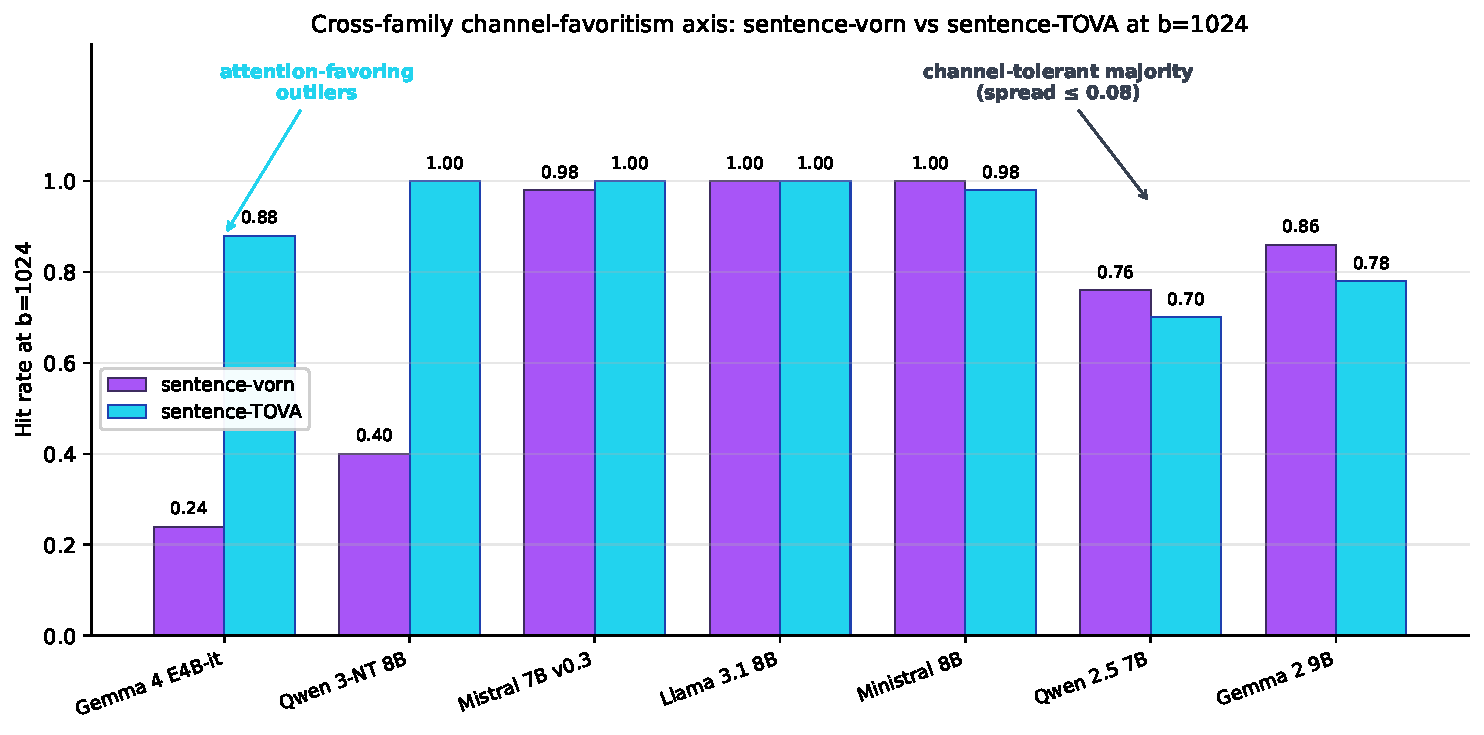
\includegraphics[keepaspectratio,alt={Cross-family channel-favoritism axis: sentence-vorn versus sentence-TOVA at budget 1024 across seven no-eviction-discriminative families. Gemma 4 and Qwen 3-NT land at the attention-favoring side; the remaining five families (Mistral, Llama, Ministral, Gemma 2, Qwen 2.5) cluster as a channel-tolerant majority with per-family spreads $\leq$ 0.08. Qwen 2.5 row reflects the post-bf16-fix re-run; the pre-fix harness run reported Qwen 2.5 as a spurious vorn-favoring extreme (Appendix C.2). The Qwen 3-NT (Qwen 3 8B with enable_thinking=False) row shows sentence-vorn rising from 0.40 at b=1024 (this figure) to 0.82-0.92 at b=1536/2048, while sentence-TOVA/H2O reach 1.000 across all three budgets --- attention-favoring shape across budgets. Qwen 3 30B-A3B is not plotted (attention-channel cells require >80GB VRAM); Gemma 3 is not plotted (observational anomaly; see Appendix C.2).}]{figures/figure1-cross-family-channel-axis.pdf}}

\textbf{Statistical methodology note.} Per-row paired McNemar tests in
this and adjacent surfaces use exact two-sided tests on discordant
pairs. Cross-family claims invoke Holm correction across the three
pre-specified rescue-spectrum primaries (Mistral + Llama + Gemma 4
family-anchored 2$\times$2 contrasts) per \S{}4.5; the three primary p-values
remain significant after correction. Anchor-grade falsification
probes (Ministral, Gemma 2, multi-budget per \S{}5.6 hybrid framing) and
the cross-family extension wave (Qwen 2.5, Qwen 3-NT) are reported
with raw p-values within local-scope families and are not promoted to
publication-strong status without their own explicit correction frame
(\S{}4.5).

\textbf{Table 1. Cross-family surface at \texttt{niah\_multikey\_1\_4k},
budget \texttt{1024}} (seven no-eviction-discriminative families on the
active claim surface). Entries are hit rates on
\texttt{niah\_multikey\_1\_4k} validation{[}:50{]}; higher is better.
"not run" indicates the method was not executed in this lane (deliberate
narrowing or runtime-unsupported; see per-family notes below the table).
Three additional families (Qwen 3 8B default-thinking, Gemma 3 12B-pt,
Qwen 3 30B-A3B) were tested with coverage limitations: Qwen 3 8B
default-thinking surfaced as drowning-floor before substrate fix
(Qwen 3-NT replaces it in the active panel under
enable\_thinking=False); Gemma 3 12B-pt vanilla is competent (1.000)
but eviction cells return 0.000 (observational anomaly); Qwen 3 30B-A3B
vanilla recovered to 1.000 under no-thinking with vorn-channel rescue
data, but attention-channel cells at b=1024 are VRAM-bounded. Both
boundary families are documented in \S{}C.2 rather than in this active
claim panel.

{\def\LTcaptype{none} % do not increment counter
{\scriptsize\setlength{\tabcolsep}{2pt}\renewcommand{\arraystretch}{0.92} \begin{longtable}[]{@{}llllllll@{}}
\toprule\noalign{}
Family & No-eviction & Token vorn & Sentence vorn & TOVA &
H2O & Sentence TOVA & Sentence H2O \\
\midrule\noalign{}
\endhead
\bottomrule\noalign{}
\endlastfoot
Mistral 7B v0.3 & 1.00\textdagger{} & 0.96\textdagger{} & 0.98\textdagger{} & 0.86\textdagger{} & 0.84\textdagger{} & 1.00\textdagger{} &
1.00\textdagger{} \\
Gemma 4 E4B-it & 1.00 & 0.02 & 0.24 & 0.94 & 0.94 & 0.88\textdaggerdbl{} & 0.86\textdaggerdbl{} \\
Llama 3.1 8B & 1.00 & 1.00 & 1.00 & 0.90 & 0.94 & 1.00\S{} & 1.00\S{} \\
Ministral 8B & 1.00 & 0.98\P{} & 1.00 & 0.44 & 0.46\P{} & 0.98\P{} & 0.98\P{} \\
Gemma 2 9B & 1.00 & 0.04\P{} & 0.86 & 0.60 & 0.60\P{} & 0.78\P{} & 0.82\P{} \\
Qwen 2.5 7B Instruct\textbar{}\textbar{} & 0.64 & 0.44 & 0.76 & 0.56 & 0.60 & 0.70 & 0.70 \\
Qwen 3-NT\textbar{}\textbar{} & 1.00 & 0.00 & 0.40 & 0.10 & 0.10 & 1.00\textdagger{}\textdagger{} & 1.00\textdagger{}\textdagger{} \\
\end{longtable}}
}

\textbf{Per-family read and statistical status} (corresponding to Table
1 rows):

\begin{itemize}
\tightlist
\item
 \textbf{Mistral}: granularity-primary family with
 vorn-robustness-to-granularity. Publication-strong: token-vorn
 dominates token-attention-weight at constrained budget (paired p $\leq$
 4.66e-10 at b=512); at b=1024 vorn lead narrows to directional (p =
 0.0625 vs TOVA, p = 0.0313 vs H2O). At sentence
 granularity all three scoring channels cluster at ceiling (paired p =
 0.5--1.0). Fresh paired n=50 surface (2026-05-19 surface); supersedes
 May 13 sweep.
\item
 \textbf{Gemma 4}: attention-favoring across the spectrum ---
 sentence-grouping does not rescue the channel-disfavored vorn at
 b=1024 (publication-strong: sentence-TOVA
 decisively beats sentence-vorn, p = 4.07e-09), but the b=256
 addendum shows sentence-TOVA at ceiling already while vorn is
 at floor, and sentence-level methods converge by b=1536. The label
 "rescue-resistant" applies at the b=1024 gate, not as a uniform
 family-wide property. Fresh paired n=50 surfaces (2026-05-19 +
 2026-05-20).
\item
 \textbf{Llama 3.1}: threshold-bounded-recovery --- full rescue at
 ceiling, partial at threshold lane. Full rescue at b=1024 (all
 sentence methods at ceiling); partial at b=256 (sentence-TOVA 0.74 vs
 sentence-vorn 1.00, p = 2.44e-04). Fresh paired n=50 (2026-05-20
 surface).
\item
 \textbf{Ministral}: same-lab architectural falsification probe + 2$\times$2
 extension. Publication-strong: 2$\times$2 at b=1024 (sentence-TOVA 0.98 vs
 token TOVA 0.44, paired p = 1.49e-08). Now extended to anchor-grade
 multi-budget coverage (b=256/512/1024/1536/2048) via 2026-05-27
 multistep-fillout; falsification-probe identity preserved (\S{}5.6).
\item
 \textbf{Gemma 2}: same-lab disambiguation probe + 2$\times$2 extension.
 Decisive paired probe + 2$\times$2 at b=1024 (sentence-TOVA 0.78 vs token
 TOVA 0.60, paired p = 0.0117). Now extended to anchor-grade
 multi-budget coverage (b=256/512/1024/1536/2048) via 2026-05-27
 multistep-fillout; falsification-probe identity preserved (\S{}5.6).
\item
 \textbf{Qwen 2.5}: channel-tolerant on this surface
 (sentence-vorn 0.76 vs sentence-TOVA 0.70 at b=1024; spread 0.06).
 Post-bf16-fix independently verified row (2026-05-26,
 0/50 fixture delta; composed artifact). Pre-fix harness run on
 2026-05-14 reported sentence-vorn 0.96 vs sentence-TOVA 0.08 as a
 spurious vorn-favoring extreme; the differential-channel-bug
 interaction is documented in Appendix C.2.
\item
 \textbf{Observational boundaries (Gemma 3 12B-pt, Qwen 3 30B-A3B)}:
 Gemma 3 12B-pt vanilla is competent (1.000) but all 18 eviction
 cells return 0.000 --- observational anomaly, deferred for mechanism
 characterization in future revision (\S{}C.2). Qwen 3 30B-A3B vanilla
 recovered to 1.000 under no-thinking config (\S{}C.2); vorn-channel
 rescue data confirms threshold-bounded recovery at MoE scale
 (sentence-vorn 0.020$\rightarrow$1.000 across b=256-2048), while
 attention-channel cells at b=1024 are VRAM-bounded (>80GB envelope).
 Qwen 3 30B-A3B serves as supporting-replication of the
 granularity-rescue mechanism at MoE scale rather than as a primary
 rescue-spectrum anchor.
\end{itemize}

\textdagger{} fresh paired n=50 Mistral 2$\times$2 surface; provenance in \S{}C.4. \textdaggerdbl{} Gemma
4 sentence-attention from 2$\times$2 + budget-fill. \S{} Llama 3.1
sentence-attention from 2$\times$2 surface. \P{} extension cells at b=1024 (now
part of anchor-grade multi-budget coverage per \S{}5.6 hybrid framing). \textbar{}\textbar{} 2026-05-20 cross-family extension wave. \textdagger{}\textdagger{} Qwen 3-NT
uses \texttt{enable\_thinking=False}; recovery status in \S{}C.2.

The panel is asymmetric: two attention-favoring families (Gemma 4 and
Qwen 3-NT) versus five channel-tolerant families (Mistral, Llama 3.1,
Ministral, Gemma 2, Qwen 2.5). See \S{}C.2
for the Qwen 2.5 post-bf16-fix correction context.

\subsection{Guardrails do not explain the Gemma and Llama split}\label{53-guardrails-do-not-explain-the-gemma-and-llama-split}

The no-guards ablation removes one obvious confound. On Gemma 4, our
TOVA and H2O baselines remain at \texttt{0.94} with or
without the prefix and recent-window scaffold, while
\texttt{sentence\_vorn} stays low (\texttt{0.24} guarded, \texttt{0.22}
unguarded) and \texttt{token\_vorn} remains collapsed (\texttt{0.02}
guarded, \texttt{0.00} unguarded). On Llama 3.1, both vorn rows remain
at \texttt{1.00} when guardrails are removed, while
TOVA and H2O stay at \texttt{0.90} and \texttt{0.94}.

This is an observational robustness check, not an equivalence proof.
What it supports is the narrower claim that the Gemma and Llama split
does not disappear when the scaffold is removed. The attention-weight
preservation on Gemma is not being carried by the guardrail, and the
vorn preservation on Llama is not either.

\subsection{Gemma 4 is a true degradation curve, not a weak negative}\label{54-gemma-4-is-a-true-degradation-curve-not-a-weak-negative}

Gemma 4\textquotesingle s budget sweep shows a bend rather than a smooth
decline. At \texttt{512}, the vorn methods are near floor
(\texttt{token\_vorn\ =\ 0.00}, \texttt{sentence\_vorn\ =\ 0.04}) while
TOVA is already at \texttt{0.34} (paired
\texttt{p\ =\ 0.000274658} versus sentence). At \texttt{1024}, the
family split becomes extreme: \texttt{sentence\_vorn\ =\ 0.24},
\texttt{token\_vorn\ =\ 0.02}, \texttt{TOVA\ =\ 0.94},
\texttt{H2O\ =\ 0.94}, with TOVA versus sentence at
\texttt{p\ =\ 5.82077e-11}. By \texttt{1536}, sentence-level retention
becomes workable (\texttt{0.68}) but still trails TOVA
(\texttt{0.98}, \texttt{p\ =\ 6.10352e-05}). By \texttt{2048},
sentence-level vorn nearly recovers the ceiling (\texttt{0.96}) while
token-level remains materially degraded (\texttt{0.52}, sentence versus
token \texttt{p\ =\ 1.04904e-05}) and TOVA saturates at
\texttt{1.00}.

The paper-safe reading is sharper than a generic negative result. Gemma
4 is not merely a family where vorn methods do less well.
It is a family where the attention-weight baseline preserves far more of
the ceiling than vorn methods at every tested budget and
nearly all of the ceiling at \texttt{1024} and above, while the
vorn ranking itself is budget-dependent and only becomes
competitive near the loosest tested budget.

\pandocbounded{\includegraphics[keepaspectratio,alt={Gemma 4 budget-sweep at 4k context (niah\_multikey\_1\_4k validation{[}:50{]}) across 6 methods $\times$ 5 budgets. Per-cell trajectories in \S{}5.3 + Table 2.}]{figures/figure2-gemma4-budget-sweep.pdf}}

\textbf{Figure 2. Gemma 4 degradation curve at 4k context} (numeric
values).

{\def\LTcaptype{none} % do not increment counter
{\scriptsize\setlength{\tabcolsep}{2pt}\renewcommand{\arraystretch}{0.92} \begin{longtable}[]{@{}lllllll@{}}
\toprule\noalign{}
Budget & Token vorn & Sentence vorn & TOVA & Sentence TOVA\textdaggerdbl{}
& H2O & Sentence H2O\textdaggerdbl{} \\
\midrule\noalign{}
\endhead
\bottomrule\noalign{}
\endlastfoot
512 & 0.00 & 0.04 & 0.34 & 0.72 & not run & 0.68 \\
1024 & 0.02 & 0.24 & 0.94 & 0.88 & 0.94 & 0.86 \\
1536 & 0.22 & 0.68 & 0.98 & 0.98 & not run & 0.98 \\
2048 & 0.52 & 0.96 & 1.00 & 1.00 & not run & 1.00 \\
\end{longtable}}
}

\textdaggerdbl{} Sentence-attention rows from Gemma 4 2$\times$2 + budget-fill surfaces
(fresh paired n=50 on current runner). Token-H2O at b=512/1536/2048 are
historical-reference rows accepted by induction from five reproducing
controls; full provenance + artifact paths in \S{}A.2 + \S{}C.4.

The sentence-attention 2$\times$2 extension supports a sharper compositional
claim about Gemma 4 than the original degradation-curve reading. At
budget 1024, sentence-attention rows beat sentence-vorn decisively
(sentence-TOVA 0.88 vs sentence-vorn 0.24, paired exact McNemar p
= 4.07e-09; sentence-H2O 0.86 vs sentence-vorn 0.24, paired p =
7.92e-09), but sentence-attention does not separate from token-attention
(sentence-TOVA 0.88 vs token TOVA 0.94, paired p = 0.453;
sentence-H2O 0.86 vs token H2O 0.94, paired p = 0.219). The
granularity transition does not change the attention-weight performance
materially. The budget-fill rows tighten this reading at the
budget tails. At budget 512, sentence-attention partially rescues the
attention-weight channel (sentence-TOVA 0.72 from token TOVA
0.34, paired exact McNemar p = 3.11e-04) while sentence-vorn collapses
(0.04); the granularity rescue is partial at the constrained-budget
tail. At budget 1536, all three sentence-level methods converge near
ceiling (sentence-vorn 0.68, sentence-TOVA 0.98,
sentence-H2O 0.98); the convergence begins one budget step earlier
than the b=2048 saturation point. By budget 2048 the ceiling-regime
sentence-level methods (vorn, TOVA, H2O) show no detected
separation in low-discordance paired tests (paired p = 0.5 to 1.0 on the
available pairs); we treat this as compatibility-with-ceiling rather
than positive equivalence evidence. At constrained budget the
family-conditional channel-favoritism persists across granularity
choices; at ceiling-regime budget the split dissolves into across-method
convergence. The Gemma 4 outlier behavior reported in
this paper is therefore \textbf{regime-bounded}, not absolute across
budgets.

\subsection{Llama 3.1 has a method-asymmetric floor}\label{55-llama-31-has-a-method-asymmetric-floor}

At the shared \texttt{1024} gate, Llama still looks easy: no-eviction,
token-level vorn, and sentence-level vorn are all \texttt{1.00}, while
TOVA and H2O drop only slightly to \texttt{0.90} and
\texttt{0.94}. The threshold cut shows why this family still matters.
Below \texttt{1024}, the methods do not degrade together. Sentence-level
vorn remains at \texttt{1.00} at \texttt{512} and \texttt{256}, with
zero discordance against the higher-budget rows. Token-level vorn stays
near the ceiling at \texttt{512} (\texttt{0.96}) but breaks at
\texttt{256} (\texttt{0.56}). The attention-weight baselines break much
harder: TOVA falls from \texttt{0.90} to \texttt{0.56} to
\texttt{0.12}, and H2O falls from \texttt{0.94} to \texttt{0.56}
to \texttt{0.08}.

This gives the Llama lane a stronger role than the original
\texttt{1024} gate alone suggested. The family is not just
threshold-shaped. It exhibits a method-asymmetric floor. Sentence-level
vorn retention remains ceiling-stable even at roughly six
percent retention, while token-level and attention-weight policies
degrade sharply. The publication-safe claim here is within-family and
budget-conditioned: on Llama 3.1, the sharp sub-\texttt{1024}
degradation appears first in the attention-weight baselines, not in
sentence-level retention.

The Phase 2A Llama 3.1 sentence-attention 2$\times$2 experiment (the 2026-05-20
Llama 3.1 2$\times$2 surface, fresh paired n=50 on current runner) resolves the
compositional question with a third distinct rescue pattern:
\textbf{threshold-bounded recovery}. At budget 1024, all sentence-level
methods converge at ceiling (sentence-vorn = 1.00, sentence-TOVA =
1.00, sentence-H2O = 1.00), consistent with the Mistral
anchor\textquotesingle s b=1024 cluster. At budget 512,
sentence-grouping delivers strong rescue of attention-weight baselines
(sentence-TOVA = 0.94 vs token TOVA = 0.56, paired exact
McNemar p = 3.81e-06, and sentence-H2O = 0.94 vs token H2O =
0.56, same rescue magnitude), while sentence-vorn holds ceiling at 1.00.
At budget 256, the rescue is partial: sentence-TOVA = 0.74 and
sentence-H2O = 0.74 (vs token TOVA = 0.12, paired p =
9.31e-10), but sentence-vorn still decisively beats sentence-TOVA
at the threshold lane (1.00 vs 0.74, paired p = 2.44e-04). The Llama
floor is therefore a sentence-vorn-specific robustness finding at
threshold budgets. Sentence-grouping rescues attention-weight
substantially but not to vorn-parity, and the rescue magnitude is
budget-dependent rather than absolute.

\S{} Phase 2A Llama 3.1 sentence-attention 2$\times$2 values from the 2026-05-20
Llama 3.1 2$\times$2 artifact. Fresh paired n=50 on current runner.

\subsection{Ministral and Gemma 2 eliminate two broad explanation classes}\label{56-ministral-and-gemma-2-eliminate-two-broad-explanation-classes}

The Ministral + Gemma 2 lanes began as targeted falsification probes
narrowly scoped to b=1024 2$\times$2 surfaces. Following the
2026-05-27 multistep-fillout extension, both lanes now carry
anchor-grade multi-budget coverage (b=256/512/1024/1536/2048 across
vorn + attention-weight methods). We keep their probe identity because
the original design rationale was hypothesis falsification rather than
rescue-spectrum anchoring; the multi-budget data extends the
falsification evidence beyond the original b=1024 gate without
reclassifying the lanes.

Ministral was the architectural-pattern test. The sentence-attention
2$\times$2 surface at b=1024 fills the family-conditional matrix beyond the
original narrow probe. Full-context no-eviction is \texttt{1.00}.
Token-level vorn \texttt{0.98}; sentence-level vorn \texttt{1.00}.
Token-level TOVA \texttt{0.44}; sentence-level TOVA \texttt{0.98}.
Sentence-grouping fully rescues the disfavored attention-weight channel
(token TOVA 0.44 $\rightarrow$ sentence TOVA 0.98, paired exact McNemar p =
1.49e-08). The
sentence-vorn vs token-TOVA contrast that drove the original narrow
probe (paired exact McNemar \texttt{p\ =\ 7.45e-09}) is now strengthened
by the full 2$\times$2 surface: the architectural-pattern falsification is
decisive across cells, not just the original probe direction.

Gemma 2 was the lab-level test. The sentence-attention 2$\times$2 surface at
b=1024 fills the family-conditional matrix beyond the original narrow
probe. Full-context no-eviction is \texttt{1.00}. Token-level vorn
\texttt{0.04} (extension-wave fill, b=1024); sentence-level vorn
\texttt{0.86}. Token-level TOVA \texttt{0.60}; sentence-level TOVA
\texttt{0.78}. Sentence-grouping
rescues the disfavored attention-weight channel (token TOVA 0.60 $\rightarrow$
sentence
TOVA 0.78, paired exact McNemar p = 0.0117). The sentence-vorn vs
token-TOVA contrast that drove the original narrow probe (paired exact
McNemar \texttt{p\ =\ 7.20e-03}) is now extended by the full 2$\times$2
surface: the lab-level falsification holds across cells.

Both probes have multi-budget coverage across b=256/512/1024/1536/2048
on the same 2$\times$2 surface, with sentence-grouping reaching ceiling
across budgets for both families. The attention-pattern-level
(Ministral) and lab-level (Gemma 2) hypotheses are decisively
falsified as sufficient explanations: both families exhibit the
channel-tolerant rescue pattern across budgets, which excludes them
from the attention-favoring class.

\subsection{Cross-task validation is bounded and task-conditional}\label{57-cross-task-validation-is-bounded-and-task-conditional}

The \texttt{qa\_2\_4k} surface does not reproduce the NIAH geometry
exactly, but it does not erase the family-conditioned split either. The
within-granularity sentence-level comparison at b=1024 (cross-task, n=200)
is the load-bearing surface here, because the original between-channel
comparison (sentence-vorn versus token-TOVA) varied on two axes
simultaneously and is not directly informative about either axis.

On Gemma 4 at sentence-level granularity: sentence-TOVA
(\texttt{0.370}, 74/200) and sentence-H2O (\texttt{0.370}, 74/200)
both decisively beat sentence-vorn (\texttt{0.260}, 52/200) on quality,
paired exact McNemar \texttt{p\ =\ 0.00209} for each comparison against
sentence-vorn. On Llama 3.1 at sentence-level granularity: sentence-vorn
(\texttt{0.460}, 92/200) versus the sentence-attention rows
(\texttt{0.425}, 85/200 for both sentence-TOVA and
sentence-H2O) shows no detected separation on this n=200 slice
(paired McNemar \texttt{p\ =\ 0.2478} for each); sentence-vorn nominally
leads but the comparison is not significant and we do not promote it to
an equivalence claim. Both sentence-attention rows beat the token-level
attention baselines (\texttt{0.330}, 66/200) at \texttt{p\ =\ 0.006609}
(within the cross-task local Holm family per \S{}4.5), confirming the
granularity rescue on the cross-task surface. On Ministral,
sentence-vorn reaches \texttt{0.510} (102/200) and sentence-attention
rows are runtime-unsupported on the current A100 stack; this is a Phase
2D stack limitation rather than a scored negative.

The cost-aware reading of this surface is developed in \S{}6.3 using the
within-channel (token versus sentence) comparison, which holds direction
and magnitude across both this cross-task surface and the primary NIAH
task. The earlier between-channel framing (sentence-vorn versus
token-TOVA on the qa\_2\_4k cost surface) is granularity-mixed and
not load-bearing for either the quality or the cost claim.

\subsection{Qwen 2.5 and Qwen 3-NT extension families}\label{58-qwen-25-7b-inverts-the-channel-favoritism-axis}

The cross-family extension wave added Qwen 2.5 and Qwen 3-NT (the
no-thinking configuration of Qwen 3 8B) to the claim-surface panel,
plus Gemma 3 12B-pt and Qwen 3 30B-A3B as observational boundaries.

\textbf{Qwen 2.5 row.} Cells at b=1024: no-eviction \texttt{0.64},
token-vorn \texttt{0.44}, sentence-vorn \texttt{0.76}, token-TOVA
\texttt{0.56}, sentence-TOVA \texttt{0.70}, token-H2O \texttt{0.60},
sentence-H2O \texttt{0.70}.

\textbf{Channel-tolerant on this surface.} Qwen 2.5 shows a small
per-family spread (sentence-vorn 0.76 vs sentence-TOVA 0.70 at b=1024,
gap \texttt{0.06}), placing it in the channel-tolerant majority of the
panel alongside Mistral, Llama 3.1, Ministral, and Gemma 2. The
asymmetric channel-favoritism finding therefore bounds to Gemma 4 and
Qwen 3-NT as the attention-favoring families; the remaining five
families are channel-tolerant.

\textbf{Multi-budget supporting evidence.} A 3-budget Qwen 2.5 surface
(b=256, b=512, b=1024) shows token-level methods floor at b=256 while
sentence-level methods rescue stably to 0.66-0.76 across all three
budgets, replicating the granularity-rescue mechanism on a fourth
family at lower no-eviction baseline (\S{}6.2).

\subsection{Provenance and supplementary analysis contract}\label{59-provenance-and-supplementary-analysis-contract}

The results above are tied to durable emitted artifacts rather than to
private run logs or chat-only summaries. The cross-family stats note
binds the surfaces it currently covers (the primary cross-family matrix
and architectural-prediction probes) to artifacts on
\texttt{origin/main}. The paired designs are preserved in row-level
observation structures, and the supplementary script
\texttt{vorn\_mat\_cross\_family\_stats.\allowbreak{}py} recomputes the paired tests
within its covered scope from the emitted rows. Claims outside the
script\textquotesingle s current coverage (the Gemma 2 fast-read, the
Llama 256-budget threshold curve, and the qa\_2\_4k cross-task surface)
are bound to their own durable artifacts with raw artifact-native
p-values. Expanding the cross-family script to cover all of Section 5 is
reproducibility-substrate future work. The paper therefore asks
reviewers to judge the claim surfaces against the same raw observation
structure the team used internally, with the caveat that re-computation
paths vary by artifact family.

\subsection{Memory Pareto frontier: vorn is cheaper, but not universally better}\label{5-10-memory-pareto-frontier}

Memory telemetry adds a second axis to the family-conditional result. On
the 7B/8B GQA rows where both vorn and attention-weight paths were
measured, attention-weight scoring is materially more memory-intensive:
Qwen 3-NT vorn peaks near 21.4 GB allocated, while Qwen 3-NT attention
rows peak near 53.3--53.8 GB allocated and 74--79.5 GB reserved; Mistral
vorn at b=1536 peaks near 20.4 GB, while H2O rows at b=1536/b=2048 peak
near 55.1--59.3 GB. Gemma 4 is a smaller-memory variant of the same
pattern: token-vorn peaks near 20.0--20.5 GB at b=1536/b=2048, while H2O
peaks near 31.3--33.2 GB.

This creates a Pareto rather than a winner-take-all frontier. Vorn can be
cheaper and retrieval-preserving on vorn-favoring families;
attention-weight rows can buy retrieval on attention-favoring families
(Qwen 3-NT sentence-attention 1.00 where sentence-vorn is 0.40; Gemma 4
attention rows saturating earlier across the rescue spectrum). OOM and
recovery statuses are part of that result: recovered rows can produce
full n=50 hit rates, but the row status signals a memory/runner
constraint that must be read alongside quality.

\pandocbounded{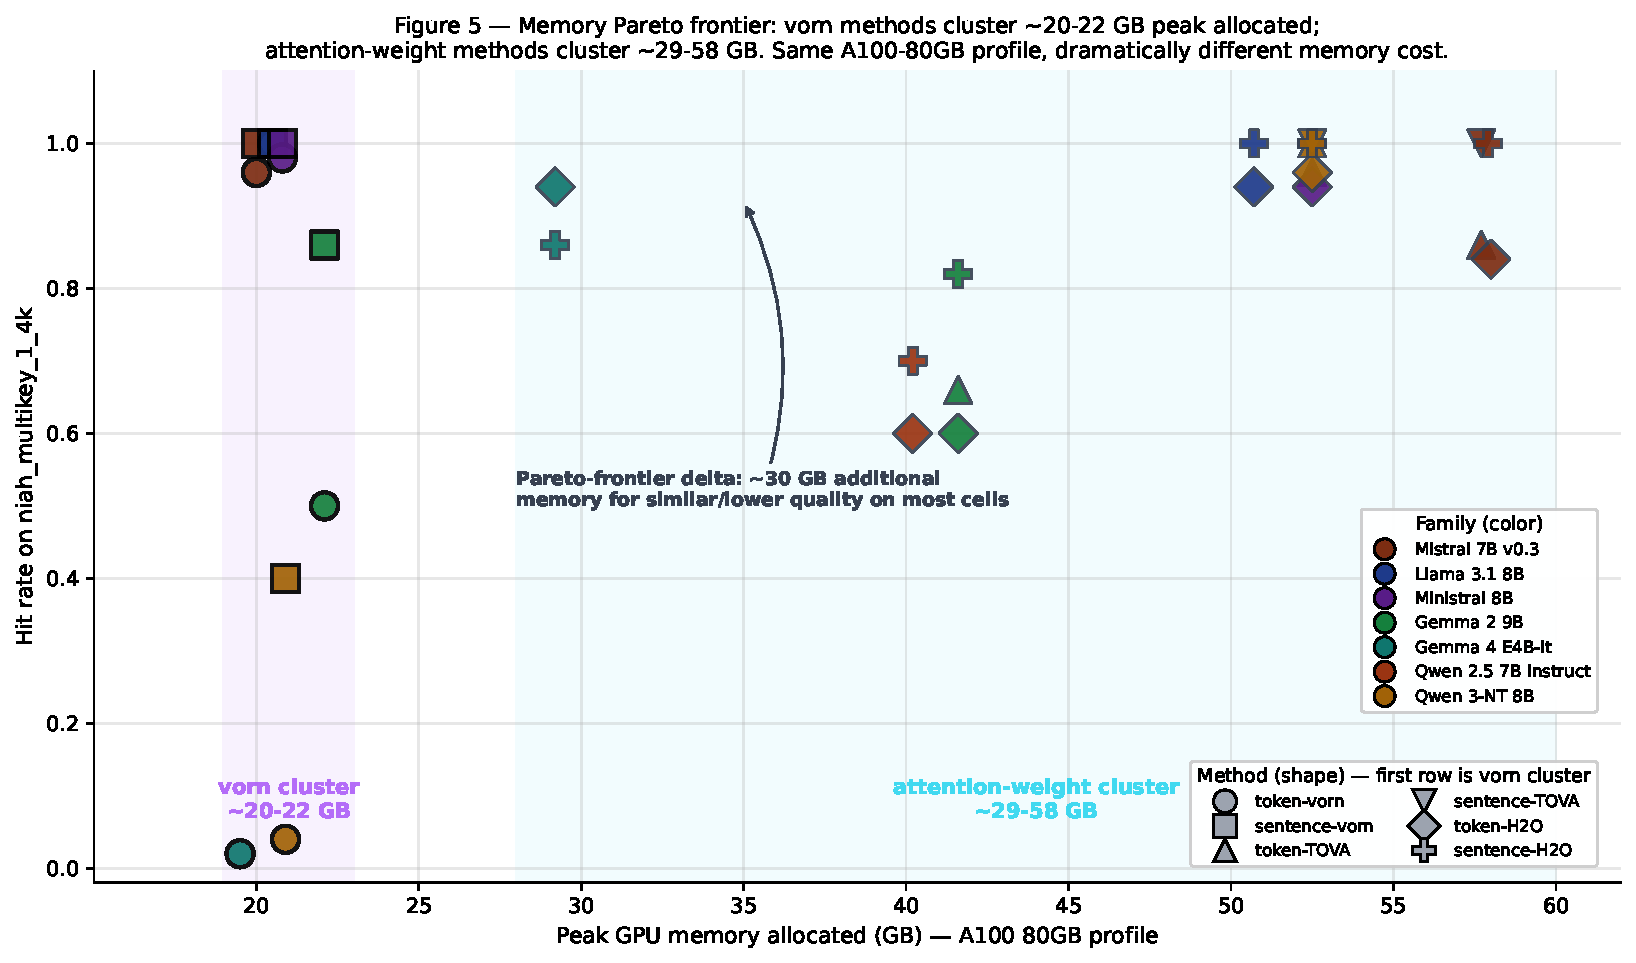
\includegraphics[keepaspectratio,alt={Memory Pareto frontier across 4k budget surfaces; each point is a (family, method, budget) cell. X-axis: peak GPU memory allocated (GB). Y-axis: hit-rate. Markers encode 6 methods; colors encode 7 families. Per-cluster analysis in \S{}5.7.}]{figures/figure5-memory-pareto.pdf}}

\begin{center}\rule{0.5\linewidth}{0.5pt}\end{center}

\section{Discussion}\label{6-discussion}

\subsection{The hypothesis space after the architectural and lab falsifications}\label{61-the-hypothesis-space-after-the-architectural-and-lab-falsifications}

The family-conditional effect described in Section 5 is asymmetric, and
its asymmetry is informative. Five of the seven families pattern together on the vorn signal, while
two families (Gemma 4 and Qwen 3-NT) pattern on the attention-weight
signal. The asymmetry rules out
symmetric explanations (such as "different scoring channels work for
different attention patterns"), because Ministral uses an interleaved
attention pattern architecturally similar to Gemma 4\textquotesingle s
and still patterns with the vorn-favoring families. The
Ministral falsification of the architectural-pattern hypothesis is
therefore directionally strong (paired McNemar p = 7.45e-09).
Post-bf16-fix Qwen 2.5 data (independently verified, Appendix C.2)
shows that family as channel-tolerant on this surface rather than as a
vorn-favoring extreme, so the attention-favoring behavior is bounded to Gemma 4 and Qwen 3-NT
within the seven-family panel. The candidate mechanism
must therefore explain why two specific families show
attention-favoring behavior while five do not.

The lab-level hypothesis is similarly falsified by Gemma 2. Same lab
as Gemma 4, but Gemma 2 patterns with the vorn-favoring
majority. If the channel-favoritism variable were at the laboratory or
training-recipe level, Gemma 2 should pattern with Gemma 4. It does not.

What remains for the Gemma 4 branch is a Gemma-4-specific
architectural or training-detail-level variable. We do not identify the specific
mechanism in this work. The candidate hypothesis space is narrower than
it was before the Ministral and Gemma 2 runs, which is the contribution
this paper can make on the mechanism question. Future work that targets
the Gemma 4 to Gemma 2 architectural or training-detail delta has a
cleaner search space because of the falsifications reported here.

The Gemma 4 outlier behavior is \textbf{granularity-asymmetric across
the rescue spectrum} (\S{}5.3, \S{}6.2): token-vorn never reaches ceiling
within tested budgets while attention-weight methods reach ceiling by
b=2048 and sentence-vorn rescue extends to near-ceiling only at the
highest tested budget. The candidate Gemma-4-specific variable must
therefore produce granularity-asymmetric channel-favoritism, ruling
out both absolute-architectural-difference and budget-uniform-
resolution hypotheses.

Qwen 3-NT broadens the hypothesis space beyond Gemma-specific
mechanisms (Table 1): its attention-favoring pattern sits on a
different lab and architecture with a configuration variable
(thinking-mode default at release). The two-family attention-favoring
class (Gemma 4 and Qwen 3-NT) broadens the mechanism search beyond
Gemma-specific candidates; targeted thinking-mode ablation is future
work (\S{}8).

A speculative candidate mechanism from \S{}5.7 + \S{}6.3: attention-weight
scoring on Gemma 4 may be both more expensive and more informative
because the interleaved attention pattern concentrates routing
information in attention statistics. Not currently testable without
targeted ablation; deferred to future work (\S{}8).

\subsection{Granularity is more load-bearing than scoring channel on the Mistral anchor family}\label{62-granularity-is-more-load-bearing-than-scoring-channel-on-the-mistral-anchor-family}

The sentence-TOVA + sentence-H2O 2$\times$2 experiment (the
2026-05-19 Mistral 2$\times$2 artifact, fresh paired n=50 on the current
runner) decomposes the granularity-versus-scoring-channel question that
single-axis comparisons cannot answer.

At token granularity, the vorn signal dominates
attention-weight scoring at the constrained budget. At budget 512,
token-vorn = 0.96 versus TOVA = 0.30 (paired exact McNemar p =
2.33e-10) and H2O = 0.32 (p = 4.66e-10). At budget 1024,
token-vorn = 0.96 versus TOVA = 0.86 (p = 0.0625) and H2O =
0.84 (p = 0.0313). The vorn-versus-attention-weight separation is
decisive at constrained budgets and narrower but still directionally
vorn-favoring at looser budgets.

At sentence granularity, the picture inverts. Sentence-vorn,
sentence-TOVA, and sentence-H2O all cluster near ceiling on this surface
(0.96-1.00 across b=512 and b=1024); paired p-values of 0.5-1.0 reflect
power-to-distinguish at near-ceiling reach, not positive equivalence.
When the retention unit is right, the scoring channel does not emerge as
the differentiating variable on this surface.

The granularity lift is asymmetric across scoring channels. Sentence
grouping moves attention-weight from collapsed (token TOVA = 0.30)
to near-ceiling (sentence TOVA = 0.96) at budget 512, a 0.66
hit-rate lift with paired p = 2.10e-09. Sentence grouping moves vorn
from already-strong (token-vorn = 0.96) to ceiling (sentence-vorn =
1.00) at budget 512, a 0.04 lift that is not paired-significant on n=50.
\textbf{Vorn is granularity-tolerant. Attention-weight is
granularity-dependent.} The unit-of-retention finding is therefore best
stated as a two-part claim. First, sentence-unit retention is the
load-bearing mechanism variable on this surface, with directionally
similar evidence across all tested scoring channels. Second,
vorn scoring is robust to granularity choice, while
attention-weight scoring requires the sentence unit to compete.

The Llama 3.1 sentence-attention 2$\times$2 (the 2026-05-20 Llama 3.1 2$\times$2
surface, fresh paired n=50 on current runner) provides direct evidence
for the granularity-primary reading on a second
vorn-favoring family with a distinct rescue profile. At
budget 256, sentence-vorn remains ceiling-stable at 1.00 while
sentence-TOVA = 0.74 and sentence-H2O = 0.74, with
sentence-vorn decisively beating sentence-TOVA (paired p =
2.44e-04). At budget 512, sentence-TOVA = 0.94 closes the gap to
sentence-vorn = 1.00 (paired p = 0.25, low power to distinguish at
near-ceiling reach). The granularity transition rescues attention-weight
substantially at all tested budgets, but not to vorn-parity at the
threshold lane.

The Gemma 4 sentence-attention 2$\times$2 (2026-05-19 artifact, fresh
paired n=50 on the current runner) tests the granularity-primary +
vorn-robustness-to-granularity pattern on the family-conditional
outlier. At budget 1024, Gemma 4 shows a structurally informative
deviation. Sentence-grouping does not rescue the channel-disfavored
signal (sentence-vorn = 0.24 versus sentence-TOVA = 0.88, paired
exact McNemar p = 4.07e-09). Sentence-attention decisively beats
sentence-vorn on Gemma 4 at b=1024. Sentence-attention does not separate
from token-attention either (sentence-TOVA 0.88 vs
token-TOVA 0.94, paired p = 0.453). Attention-weight is already
granularity-tolerant in its favored channel on Gemma 4. At budget 2048
the picture converges: all sentence-level methods cluster near ceiling
(sentence-vorn 0.96, sentence-TOVA 1.00, sentence-H2O 1.00)
with no decisive separation (paired p = 0.5 to 1.0). At constrained
budget the family-conditional channel-favoritism persists across
granularity choices. At ceiling-regime budget it dissolves into
across-method convergence.

\pandocbounded{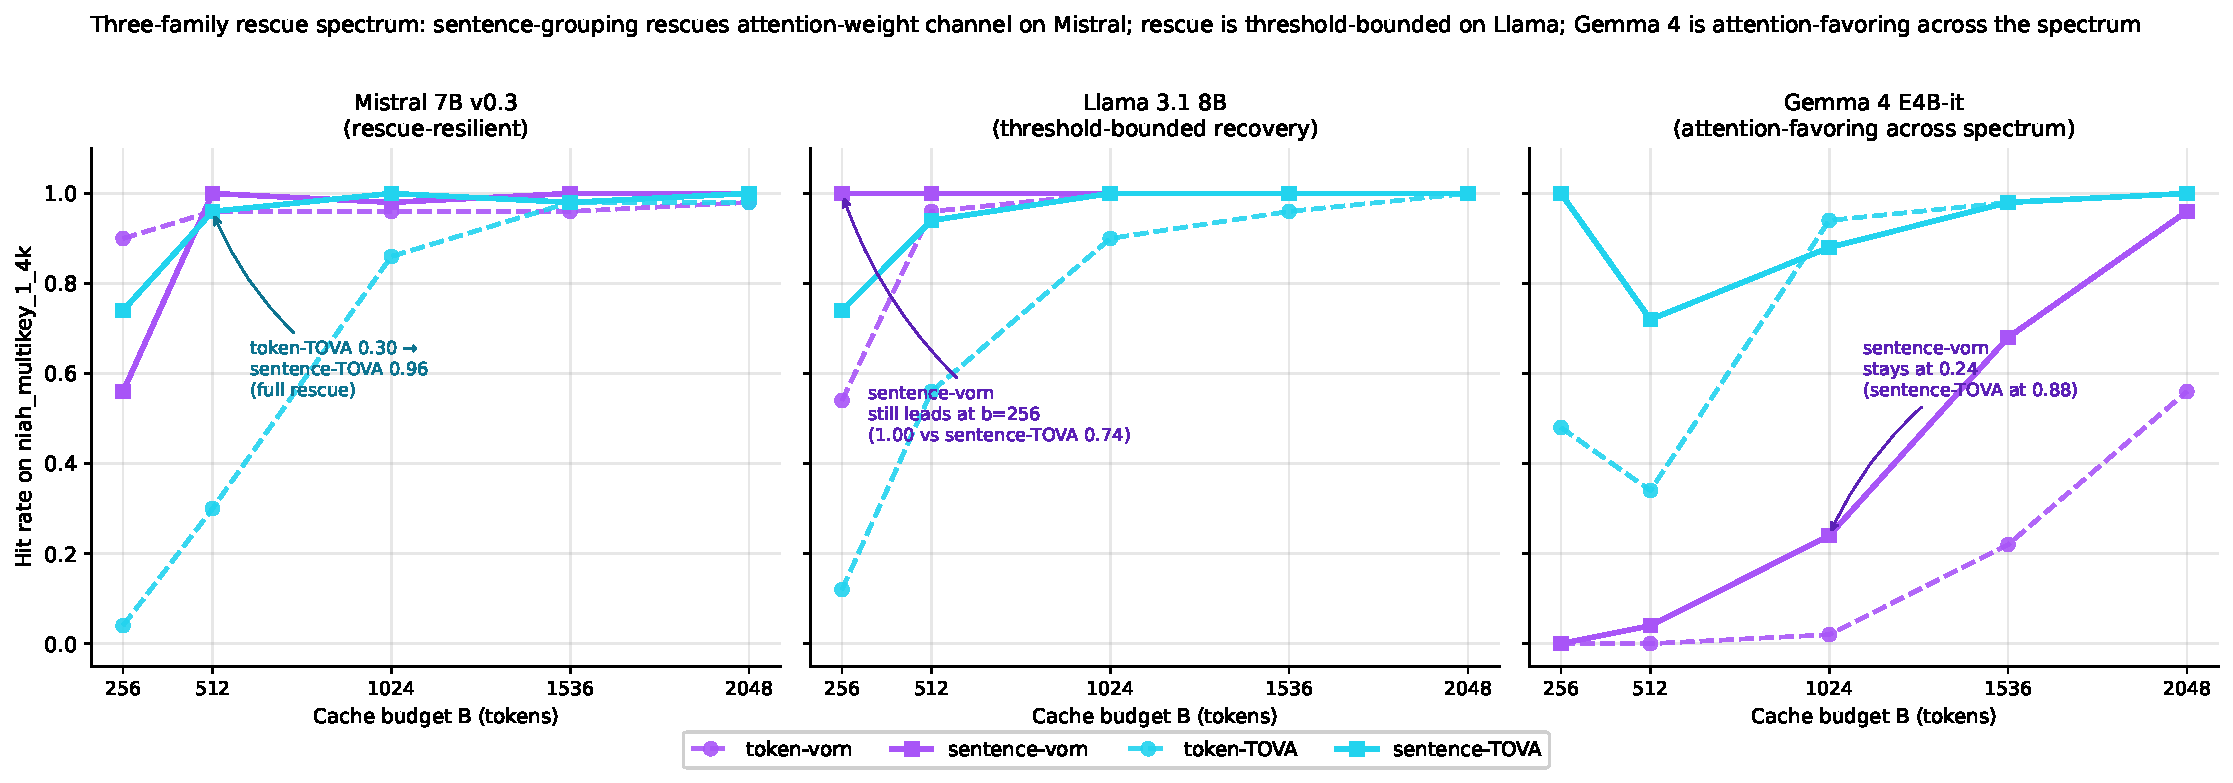
\includegraphics[keepaspectratio,alt={Three-panel rescue spectrum across Mistral (rescue-resilient), Llama (threshold-bounded recovery), and Gemma 4 (attention-favoring across spectrum) 2$\times$2 surfaces; scoring-channel $\times$ granularity-unit versus cache budget on niah\_multikey\_1\_4k at b $\in$ \{256, 512, 1024, 1536, 2048\}. Per-panel discussion in \S{}6.2; TOVA-only on Mistral + Llama (H2O multi-budget exists only on Gemma 4 per Figure 2).}]{figures/figure3-rescue-spectrum.pdf}}

The compositional read across three family-anchored 2$\times$2 surfaces
(Mistral 2$\times$2 surface (2026-05-19), Gemma 4 2$\times$2 surface (2026-05-19),
Llama 3.1 2$\times$2 surface (2026-05-20)) reveals a \textbf{rescue spectrum}
rather than a binary class property. Three distinct rescue profiles
emerge. \textbf{Rescue-resilient on Mistral}: full rescue across the budget
spectrum (attention-weight 0.30$\rightarrow$0.96 at b=512). The late-budget Mistral
attention-weight cells at b=1536 and b=2048 are filled via 3-case
micro-recovery composition (\texttt{completed\_recovered}; see
Appendix C.3) and confirm rescue-resilient behavior holds across the
full b $\in$ \{256, 512, 1024, 1536, 2048\} range.
\textbf{Threshold-bounded recovery on Llama}: strong rescue at b=512
with sentence-TOVA 0.94 vs token 0.56, partial rescue at b=256 where
sentence-vorn 1.00 still decisively beats sentence-TOVA 0.74
(p = 2.44e-04). \textbf{Attention-favoring across the spectrum on
Gemma 4}: sentence-grouping does not rescue vorn at b=1024
(0.02$\rightarrow$0.24), and the family-conditional split persists across
granularity choices at constrained budgets; at b=2048 the split
dissolves into across-method convergence. The channel-favored
scoring signal is granularity-tolerant on all three families (vorn on
Mistral and Llama, attention-weight on Gemma 4). The family-conditional
channel-favoritism is robust to granularity-grouping at constrained
budgets and dissolves at ceiling-regime budgets. This is a
\textbf{regime-bounded} spectrum finding rather than an absolute
family-wide split, and the rescue-threshold position varies by family.

The Ministral and Gemma 2 2$\times$2 surfaces now carry anchor-grade
multi-budget coverage (b $\in$ \{256, 512, 1024, 1536, 2048\} across vorn
+ attention-weight methods) following the 2026-05-27 multistep-fillout
extension. They retain their falsification-probe identity from the
original Phase 2B design (\S{}5.6 hybrid framing). The three primary
rescue-spectrum anchors (Mistral, Llama 3.1, Gemma 4) carry full
multi-budget 2$\times$2 coverage after the 2026-05-20 budget-fill spans b $\in$
\{256, 512, 1024, 1536, 2048\} on all three families. The Mistral panel includes b=256 +
512 + 1024 + 1536 + 2048 across all four methods; the attention-weight
rows at b=1536 and b=2048 are filled via 3-case micro-recovery
composition (Appendix C.3) per the 2026-05-26 budget-fill wave.
The Llama panel includes all five budgets across all four methods. The
Gemma 4 panel includes all five budgets across all four methods, with
the b=256 addendum showing sentence-TOVA at ceiling (50/50) while both
vorn rows remain at floor (0/50 each). The unit-of-retention finding is
therefore established on three full multi-budget 2$\times$2 surfaces with
distinct rescue profiles and extended with two anchor-grade
falsification-probe confirmations (Ministral + Gemma 2, multi-budget
per \S{}5.6 hybrid framing), but the full-budget-range class claim
remains anchored on the three primary rescue-spectrum surfaces. Qwen 3
8B does not exhibit a sentence-granularity advantage on the tested slice
(drowning-floor regime, no-eviction = 0.00), so the finding is also
explicitly model-bounded. The supported claim is a three-family rescue
spectrum: sentence-unit retention is a first-class mechanism variable;
rescue magnitude is family- and budget-conditioned; the channel-favored
signal is granularity-tolerant within the tested cells; and untested
families and fast-read probes remain outside the class claim.

\textbf{Qwen 2.5 multi-budget supporting evidence (replication, not
fourth anchor).} The post-bf16-fix Qwen 2.5 refresh on the canonical
harness (2026-05-26; Appendix C.2) extends Qwen 2.5 to three budgets
(b=256, b=512, b=1024 on \texttt{niah\_multikey\_1\_4k}; no cross-task
parity). The data shows a granularity-rescue pattern: token-level
methods floor or near-floor at b=256 (token-vorn 0.00, token-TOVA 0.14,
token-H2O 0.12) while sentence-level methods rescue stably across
budgets (sentence-vorn / sentence-TOVA / sentence-H2O cluster in
0.66-0.76 across b=256/512/1024 with per-family spread $\leq$ 0.06). The
shape replicates the granularity-rescue mechanism on a fourth family at
a lower no-eviction baseline (0.64), with the notable difference vs
Mistral that the rescue extends to vorn-channel cells as well, not just
attention-weight cells --- consistent with \S{}6.2's headline that
granularity is more load-bearing than scoring channel. The Qwen 2.5
panel is reported as supporting replication of the rescue mechanism
rather than as a fourth primary spectrum anchor: it has 3-budget
coverage (not 5), no cross-task validation surface, and a
capability-bounded ceiling that limits comparability with the
multi-budget anchor surfaces. The 3-family rescue spectrum remains the
claim-tier-strong scaffold.

\textbf{Qwen 3 30B-A3B MoE-scale supporting evidence.} A 5-budget
Qwen 3 30B-A3B eviction panel on the canonical bf16 harness
(Appendix C.2) demonstrates that granularity-rescue applies at MoE
scale (3B-active / 30B-total parameters). Sentence-vorn shows sharp
threshold-bounded recovery across budgets (0.020 $\rightarrow$ 0.020
$\rightarrow$ 0.420 $\rightarrow$ 0.980 $\rightarrow$ 1.000 across
b=256/512/1024/1536/2048), with the b=1024-to-b=1536 threshold sharper
than the three rescue-spectrum anchors. Token-vorn floors completely
at all tested budgets --- granularity is the load-bearing rescue
variable here as well. Attention-channel methods at b=1024 are
VRAM-bounded ($>$80GB required; full coverage deferred to v2). Qwen 3
30B-A3B is included as supporting-replication of the granularity-rescue
mechanism at MoE scale rather than as a fourth primary spectrum anchor.

\subsection{Granularity is cost-dominant --- within every scoring channel}\label{63-granularity-is-cost-dominant--within-every-scoring-channel}

The cost-aware framing of the family-conditional finding turns on a
within-channel comparison rather than a between-channel one. Holding the
scoring channel constant (vorn, or TOVA, or H2O) and varying
only the retention granularity (token-level versus sentence-level),
sentence-grouping reduces cost per correct answer in every non-floor
non-anomalous within-channel cell measured at the reported cost surfaces
(the explicit exclusions and their underlying numbers are listed in the
Figure 4 caption and Appendix A.7).

\pandocbounded{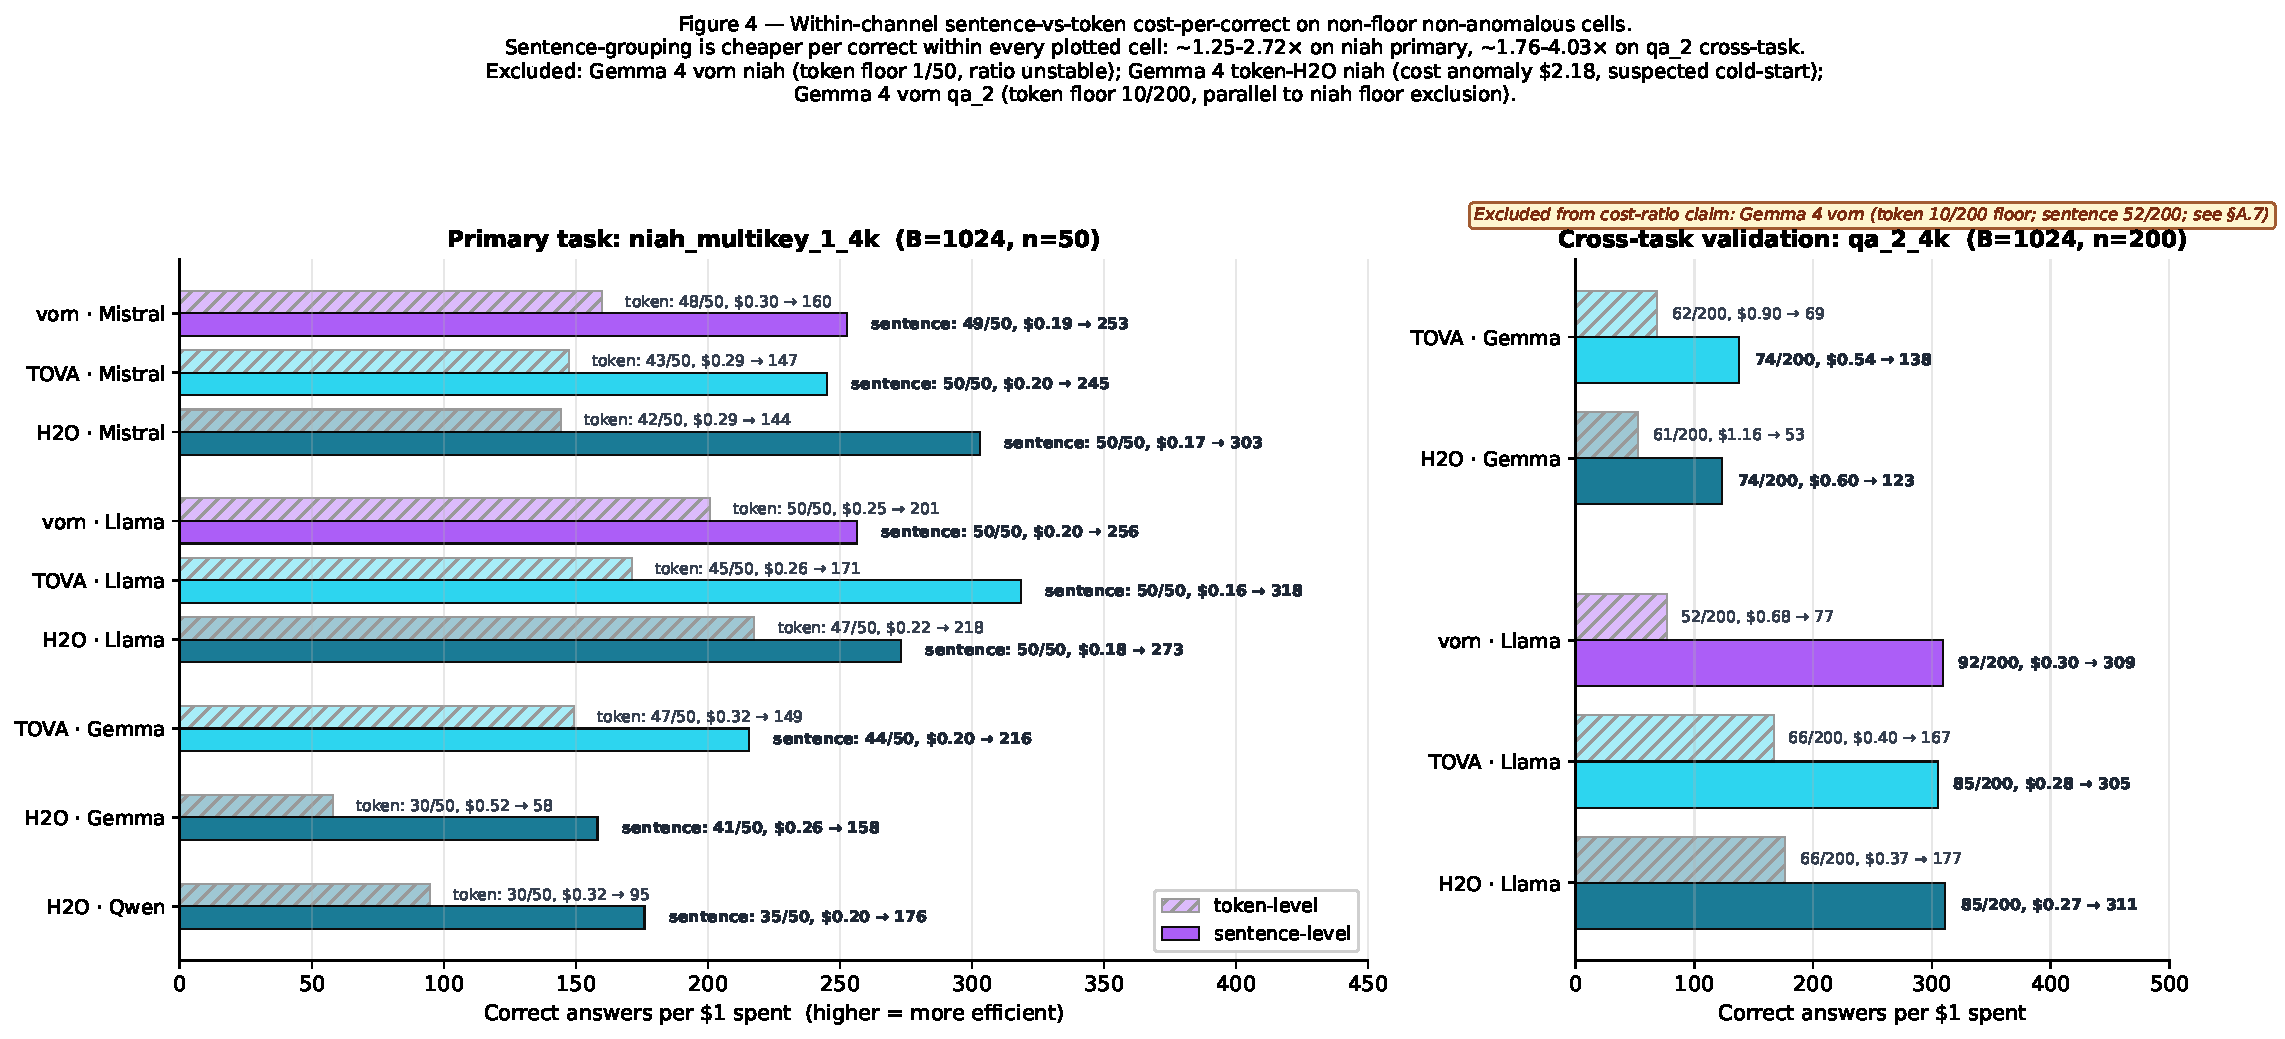
\includegraphics[keepaspectratio,alt={Within-channel sentence-vs-token cost-per-correct on the primary task (niah\_multikey\_1\_4k at B=1024, n=50, left panel) and cross-task validation surface (qa\_2\_4k at B=1024, n=200, right panel). For each (family, scoring channel) cell, paired bars show correct answers per dollar spent at token-level (hatched) versus sentence-level (solid). Sentence-grouping is cheaper per correct answer in every plotted cell: ~1.25-2.72$\times$ on the primary task, ~1.76-4.03$\times$ on cross-task. Excluded cells (floor or cost-anomaly) and full per-cell derivation in \S{}A.7.}]{figures/figure4-cost-quality-scatter.pdf}}

On the primary task, the within-channel cost comparison reads cleanly
across families. On Mistral:
token-vorn 48/50 at \$0.300 (160 correct per \$1) versus
sentence-vorn 49/50 at \$0.194 (\textbf{253 correct per \$1}, 1.6$\times$
cheaper per correct); token-TOVA 43/50 at \$0.292 (147) versus
sentence-TOVA 50/50 at \$0.204 (\textbf{245}, 1.7$\times$ cheaper);
token-H2O 42/50 at \$0.291 (144) versus sentence-H2O 50/50
at \$0.165 (\textbf{303}, 2.1$\times$ cheaper). On Llama 3.1: token-vorn
50/50 at \$0.249 (201) versus sentence-vorn 50/50 at \$0.195
(\textbf{256}, 1.3$\times$ cheaper); token-TOVA 45/50 at \$0.263 (171)
versus sentence-TOVA 50/50 at \$0.157 (\textbf{318}, 1.9$\times$
cheaper); token-H2O 47/50 at \$0.216 (218) versus
sentence-H2O 50/50 at \$0.183 (\textbf{273}, 1.3$\times$ cheaper). On
Gemma 4: token-TOVA 47/50 at \$0.315 (149) versus
sentence-TOVA 44/50 at \$0.204 (\textbf{216}, 1.5$\times$ cheaper). Only
one (family $\times$ channel) cell is plotted for Gemma 4 on the primary task
because the other two channels are outlier cells excluded from the
within-channel ratio summary: the Gemma 4 vorn channel is a floor case
(token-vorn 1/50, ratio unstable near zero), and the Gemma 4 token-H2O
cost is anomalous at \$2.180 versus \textasciitilde\$0.30 on adjacent
token-attention cells (suspected Modal cold-start cost-recording
artifact; flagged for re-verification in \S{}A.7). The Option C H2O
extensions (\S{}5.2) set the upper end of the primary-task range. On
Gemma 2: token-H2O 30/50 at \$0.5166 (58 correct per \$1) versus
sentence-H2O 41/50 at \$0.2592 (\textbf{158}, 2.72$\times$ cheaper), which
is the strongest single-cell sentence-cheaper-than-token ratio on the
primary task. On Qwen 2.5: token-H2O 30/50 at \$0.3169
versus sentence-H2O 35/50 at \$0.1989 (1.86$\times$ cheaper). Both excluded
cells are documented in the Appendix A.7 honest-negatives list with the underlying
numbers preserved for transparency; the cost-ratio claim summarized in
the abstract and Figure 4 caption is scoped to non-floor non-anomalous
cells, consistent with this exclusion.

On the cross-task surface, the
pattern holds in the same direction with similar magnitudes. On Gemma 4: token-TOVA 62/200 at
\$0.8995 (69 correct per \$1) versus sentence-TOVA 74/200 at
\$0.5375 (\textbf{138}, 2.0$\times$ cheaper); token-H2O 61/200 at
\$1.1577 (53) versus sentence-H2O 74/200 at \$0.5997
(\textbf{123}, 2.3$\times$ cheaper). On Llama 3.1: token-TOVA 66/200
at \$0.3954 (167) versus sentence-TOVA 85/200 at \$0.2789
(\textbf{305}, 1.8$\times$ cheaper); token-H2O 66/200 at \$0.3738 (177)
versus sentence-H2O 85/200 at \$0.2732 (\textbf{311}, 1.8$\times$
cheaper). Four cells across two families on the harder cross-task
surface, all four sentence-cheaper-than-token with consistent magnitude.

The mechanism is structural rather than empirical. Sentence-level
retention scores fewer items per eviction decision (sentence-pooled
candidates rather than individual tokens), and the cache writeback
overhead drops accordingly. The cost reduction does not depend on which
scoring channel produces the per-sentence summary; it depends on the
granularity of the eviction decision itself.

The scoring channel choice (vorn versus TOVA/H2O) does
\textbf{not} produce a systematic cost-per-correct advantage at
sentence-level granularity. On Gemma 4 cross-task at B=1024 the
within-granularity comparison shows sentence-TOVA (74/200 at
\$0.5375) and sentence-H2O (74/200 at \$0.5997) both decisively
beat sentence-vorn (52/200 at \$0.4620) on quality (paired exact McNemar
p = 0.00209 for each within the cross-task local Holm family per \S{}4.5),
and correspondingly on observed cost-per-correct (138 and 123 versus 113
per \$1). On Llama 3.1 cross-task at B=1024, sentence-vorn (92/200 at
\$0.2976), sentence-TOVA (85/200 at \$0.2789), and
sentence-H2O (85/200 at \$0.2732) show no detected quality
separation on this n=200 slice (paired McNemar p = 0.2478 for each
comparison against sentence-vorn) with sentence-vorn nominally leading;
observed cost-per-correct values cluster tightly at 309, 305, 311 per
\$1. Cost-per-correct values are reported as descriptive run-measured
ratios, not as inferential statistics --- McNemar tests apply to the
paired quality outcomes, not to the cost ratios. The cost-per-correct
ratio is informative only where methods produce nonzero hit rates; in
drowning-floor regimes the ratio is ill-defined.

This composes with \S{}6.2 rather than competing with it. The
unit-of-retention variable is load-bearing on two axes simultaneously:
it determines the rescue magnitude (\S{}6.2, family-conditional) and it
determines the cost-per-correct ratio (\S{}6.3, family-uniform within the
measured cells). The two findings reinforce each other and point at the
same operational recommendation: in cost-sensitive deployments,
sentence-grouping is the high-leverage configuration choice, regardless
of which scoring channel a family\textquotesingle s mechanism favors.
The earlier between-channel framing --- comparing sentence-vorn against
token-TOVA on the cross-task surface --- varied on two axes
simultaneously and is not load-bearing here; the within-channel
comparison reported above is the surface that carries the cost finding.

We treat this cost-aware analysis as a methodological contribution to
the eviction literature in its own right. The prior art surveyed in
Section 2 typically reports quality results without normalizing for
inference cost across methods. The within-channel sentence-vs-token cost
surface is a missing axis in the public literature; reporting it makes
the granularity-as-mechanism finding (\S{}6.2) operationally legible to
deployment teams.

\subsection{Implications for hierarchical inference systems and capacity-constrained inference}\label{64-implications-for-hierarchical-inference-systems-and-capacity-constrained-inference}

The family-conditional finding has direct implications for two adjacent
system classes. Hierarchical inference systems (InfLLM, InfiniGen,
Activation Beacon, Quest) make substrate-selection decisions at scale
across pre-computed embeddings or paged KV state. The scoring criterion
within their substrate selection is typically attention-statistical or
query-projection-based. The family-conditional channel-favoritism
finding reported here suggests their substrate-selection rules should be
family-conditional as well, with vorn-conditioned variants
worth testing on the vorn-favoring families.

Capacity-constrained inference (small-model serving, edge deployment,
capacity-throttled tiers within production stacks) is the other
implication surface. The \S{}6.3 finding identifies sentence-grouping as
the cost-dominant configuration choice across families and scoring
channels, which is directly actionable for high-volume serving
regardless of family. A second structural observation is relevant for
memory-constrained deployment. Let \texttt{L} denote the prefill
sequence length (number of tokens scored during the one-shot
prefill-time eviction decision). When the attention-weight scoring path
materializes the full \texttt{L\ $\times$\ L} prompt attention matrix to
aggregate importance across heads --- which is required when
flash-attention kernels cannot be used to fuse aggregation with the
attention computation, as is the case in our prototype runner --- its
\textbf{peak} prefill-time intermediate scales as
\texttt{O(L\ $\times$\ L\ $\times$\ heads)}. Vorn scoring\textquotesingle s peak intermediate is
\texttt{O(L\ $\times$\ d\_model)} because it requires only the canonical
hidden-state at the mid-depth layer \texttt{L*=L//2}. The
quadratic-in-\texttt{L} cost on the attention-weight path therefore
depends on the flash-attention-incompatible materialization step; on
runners that fuse the aggregation, the peak memory profile would be
lower (accumulated-statistics buffers scale closer to
\texttt{O(L\ $\times$\ heads\ $\times$\ layers)}, not \texttt{O(L\ $\times$\ L\ $\times$\ heads)}).
Constants omitted from these expressions (layer count, batch size, dtype
precision, per-head dimension, intermediate dtype during aggregation)
are runner-dependent and not part of the structural prediction itself.
The Mistral budget-fill experiment at b=1536 and b=2048
documented a concrete consistent instance: vorn methods
(token-vorn, sentence-vorn) completed cleanly on H100 80GB, while
attention-weight methods (TOVA, sentence-TOVA) hit CUDA OOM
at the same budgets on the same hardware (2026-05-20 Mistral
budget-fill; attention-weight rows subsequently recovered via 3-case
micro-recovery composition, Appendix C.3). We
treat this as a qualitative architectural observation consistent with
the structural intermediate-size prediction under our prototype
runner\textquotesingle s flash-attention-incompatible materialization
step rather than a quantified memory model; instrumented memory
measurement is reserved for future work (\S{}6.10).

\subsection{Cross-task generalization}\label{65-cross-task-generalization}

The cross-family matrix described in Section 4 tested
\texttt{niah\_multikey\_1\_4k} as the primary slice. Cross-task
validation on \texttt{qa\_2\_4k} was then run on Gemma 4, Llama 3.1, and
Ministral at \texttt{n\ =\ 200}. The family-conditioned split does
not disappear on this task. Gemma\textquotesingle s best completed
compressed rows remain attention-weight methods. Llama\textquotesingle s
best completed compressed row remains sentence-level vorn.
Ministral\textquotesingle s completed sentence row stays near
no-eviction, while the attention-weight rows were runtime-unsupported on
the current stack.

The absolute gaps are smaller than on the NIAH slice, and only some
paired comparisons are decisive. The supported claim is therefore
narrower than a second full family map. The cross-task surface is
compatible with the family-conditioned reading, but it does not
establish a universal task-invariant law. Cross-task validation remains
bounded and observational, and the natural next step is broader
multi-task replication rather than stronger wording on the current
surface.

\subsection{Honest negatives sharpen the claim}\label{66-honest-negatives-sharpen-the-claim}

Several negative results materially shaped the argument: the paired-
test correction moved the inferential layer to exact McNemar; the Qwen
3 8B drowning-floor blocked a universal sentence-law claim; the Gemma
4 outlier blocked a universal vorn-superiority claim; the online
adaptive selector failure blocked a premature real-time-policy claim.
None weakened the research program; together they carved away weaker
or unjustified forms of the claim and left a smaller, more credible
core. \S{}6.7 enumerates what the current evidence does and does not
support; \S{}A.7 carries the artifact-level honest-negative ledger.

\subsection{What the current evidence does and does not support}\label{67-what-the-current-evidence-does-and-does-not-support}

The following framing extends to the cross-family expansion:

\textbf{Supported by the current evidence}:

\begin{itemize}
\tightlist
\item
 KV-cache eviction effectiveness is family-conditional across the
 seven-family panel. Gemma 4 and Qwen 3-NT are the attention-favoring
 families; five families (Mistral, Llama, Ministral, Gemma 2,
 Qwen 2.5) are channel-tolerant on the b=1024 surface.
\item
 Attention-pattern and laboratory-identity are decisively falsified
 as sufficient explanations for the channel-favoritism variable
 (Ministral + Gemma 2 probes). The remaining candidate space is a
 model-specific architectural, training, or configuration variable
 that may differ across the two attention-favoring families
 (Gemma 4 branch: architectural/training-detail; Qwen 3-NT branch:
 configuration variable such as thinking-mode default).
\item
 Across three family-anchored sentence-attention 2$\times$2 surfaces,
 sentence-unit retention is a first-class mechanism variable: Mistral
 rescue-resilient, Llama threshold-bounded recovery, Gemma 4
 rescue-resistant for the disfavored vorn channel. Qwen 2.5 multi-
 budget data replicates the granularity-rescue mechanism at
 lower-capability bound (\S{}6.2).
\item
 Sentence-grouping reduces cost per correct answer within every
 non-floor non-anomalous (family, scoring channel) cell measured:
 1.25-2.72$\times$ on the primary NIAH task and 1.76-4.03$\times$ on cross-task
 \texttt{qa\_2\_4k} (strongest single-cell descriptive ratio: Llama 3.1
 vorn cross-task at 4.03$\times$; the corresponding paired quality
 comparison is significant at p = 1.03e-08). The cost finding concerns
 granularity, not scoring channel. Outlier and floor cells are
 excluded from the cost-ratio summary and footnoted in \S{}A.7.
\item
 The qa\_2\_4k surface is compatible with the family-conditioned
 reading on completed rows, with task-conditional magnitude; it is
 not a full cross-task generalization.
\end{itemize}

\textbf{Not supported by the current evidence}:

\begin{itemize}
\tightlist
\item
 A universal cross-family law of vorn superiority.
\item
 A universal cross-family law of sentence-granularity superiority.
\item
 A claim that the adaptive hypothesis has already been operationalized
 as a viable online selector.
\item
 A specific identification of the Gemma-4-specific architectural
 variable.
\item
 A claim about behavior beyond 4k context (8k validation exists only on
 Mistral, and 16k not validated due to RULER mirror contamination).
\end{itemize}

\subsection{Limitations}\label{68-limitations}

We note the limitations explicitly.

\begin{itemize}
\tightlist
\item
 \textbf{Sample size}: n = 50 per row on most cells, n = 200 on
 cross-task. The asymmetric attention-favoring claim across seven
 families (five channel-tolerant, two attention-favoring on Gemma 4
 and Qwen 3-NT) at 50 fixtures relies on Wilson CIs and paired
 McNemar tests at every comparison. Larger-sample validation is
 future work.
\item
 \textbf{Single benchmark family}: RULER. Cross-benchmark
 generalization is open.
\item
 \textbf{Single context length on most cells}: 4k. We make no
 load-bearing longer-context claim beyond 4k. Older Mistral 8k results
 referenced in earlier drafts are provenance-only pending same-runner
 refresh and are not used to support any claim in this paper.
\item
 \textbf{Seven families, all no-eviction-discriminative}: meaningful
 for a cross-family analysis, but not exhaustive. Coverage gaps
 include additional no-eviction-discriminative MoE families (Qwen 3
 30B-A3B vanilla recovered to 1.000 under no-thinking with
 vorn-channel rescue data; attention-channel cells at b=1024 are
 VRAM-bounded; preserved in \S{}C.2 as supporting-replication), larger
 models beyond 12B, and non-English-primary models.
\item
 \textbf{Mechanism unidentified}: we falsify attention-pattern and
 laboratory-identity as sufficient explanations but do not positively
 identify the Gemma-4-specific variable.
\item
 \textbf{Attention-weight baselines are same-runner approximations, not
 author-code-verified reproductions}: TOVA \citep{oren2024tova} and H2O
 \citep{zhang2023h2o} are reimplementations of the published scoring
 contracts within our runner. Internal determinism is verified (replay
 reproduces bit-exact scores on Mistral 7B / niah\_multikey\_1\_4k /
 b=1024 / n=200). Author-code reproduction was attempted on all
 families; only Mistral was achievable (Gemma 4 fails at
 \texttt{KeyError(\textquotesingle{}gemma4\textquotesingle{})}, Llama
 3.1 fails at \texttt{rope\_scaling} validation). On Mistral, author-code
 TOVA reached 50/50 versus our same-runner \texttt{tova\_1024\_guarded}
 at 43/50 (paired exact McNemar p = 0.0156, one-directional 7-cell
 gap), with the caveat that the comparator includes guardrail +
 recent-window scaffolding that the author-code does not. Our
 implementation is faithful-direction-but-slightly-conservative on the
 one family where author-code permits comparison.
 Family-dependent implementation-faithfulness on Gemma 4, Llama 3.1,
 Qwen 2.5, and Qwen 3-NT is untested and is a partial-explanation
 hypothesis we cannot rule out. Section 5 should therefore be read as
 "vorn versus our same-runner attention-weight controls." Cross-family
 author-code verification is in \S{}8.3.
\item
 \textbf{Budget-curve cross-runner boundary for Mistral}: Mistral
 b=256--1024 ran on A100 80GB; b=1536 and b=2048 ran on H100 80GB after
 A100 OOMed on attention-weight rows. Hit-rate is theoretically
 runner-invariant under deterministic harness (replay reproduces
 bit-exact), but cross-runner trajectory interpretation carries an
 unbounded comparability assumption we cannot empirically verify
 without an A100 re-run. Cost-per-correct values are runner-dependent
 (Modal A100 80GB and H100 80GB billed at different rates) and recorded
 per-artifact for downstream re-aggregation. The
 \textbf{rescue-resilient on Mistral} framing rests on n=50 data
 across all budgets. Llama 3.1 and Gemma 4 panels are single-runner;
 the cross-runner caveat does not extend to those panels. See \S{}C.4
 for substrate-evolution context (including micro-recovery
 composition methodology and its small-n divergence boundary at
 b=256 sentence-H2O).
\end{itemize}

The \S{}6 supplementary cell (Mistral-anchored vorn vs
SnapKV-style/PyramidKV-style/Quest-style) extends this same-runner
methodology to three additional newer KV-cache eviction methods. We
could not run the official upstream repositories of these methods on our
infrastructure because each is tied to incompatible transformers
versions (similar to the TOVA author-code stack incompatibility above).
We therefore reimplemented each method\textquotesingle s scoring
contract within our experimental runner under identical guardrails and
budget enforcement. The cell reports sentence-vorn 0.98 vs SnapKV-style
0.46 (paired exact McNemar p = 2.98e-08), PyramidKV-style 0.84 (p =
0.0391), Quest-style 0.54 (p = 2.98e-06). The same caveat applies:
these are same-runner reimplementations of each method\textquotesingle s
scoring contract, not author-code reproductions; absolute-benchmark
positioning against published numbers is open and tracked in \S{}8.3.

\begin{itemize}
\tightlist
\item
 \textbf{Online adaptive selector v0 failed}: the post-hoc regime map
 identifies where an adaptive policy is worth trying, but the v0
 selector is not it.
\end{itemize}

\subsection{Production implication}\label{69-production-implication}

The production implication, in the bounded form the current evidence
supports, is:

\begin{enumerate}
\def\labelenumi{\arabic{enumi}.}
\tightlist
\item
 Treat unit-of-retention as a first-class mechanism variable in the
 eviction substrate.
\item
 Expect the best scoring channel and the best unit to depend on budget
 regime and model family.
\item
 Prefer sentence-level retention where cost-per-correct is the
 operative metric on completed nonzero cells. Choose the scoring
 channel by family and quality target --- vorn for vorn-favoring
 families (Mistral, Llama 3.1, Ministral, Gemma 2), attention-weight
 for the Gemma 4 outlier where the disfavored vorn channel does not
 rescue under sentence-grouping. Qwen 2.5 is channel-tolerant on this
 surface (per-family spread 0.06); either scoring channel is
 acceptable.
\item
 Preserve paired, per-fixture evaluation artifacts so future adaptive
 policies can be judged against the same exact cases.
\end{enumerate}

\subsection{Next empirical moves}\label{610-next-empirical-moves}

The following framing organizes the read:

\begin{itemize}
\tightlist
\item
 Targeted ablation on the Gemma 4 to Gemma 2 architectural or
 training-detail delta to identify the channel-favoritism variable
\item
 Observation-level score-distribution work to design a better online
 adaptive selector than peak-zscore-over-current-alignment
\item
 Broader cross-model testing on additional MoE families and larger
 model scales as cleaner model access becomes available
\item
 Cross-benchmark validation beyond RULER (LongBench, InfiniteBench)
\item
 Broader multi-task replication beyond qa\_2\_4k (where n=200 supports
 the family-conditioned reading decisively on Llama, directionally on
 Gemma, with some Ministral attention rows runtime-unsupported on the
 current evaluation stack)
\item
 \textbf{Instrumented peak-GPU-memory measurement per scoring path.}
 The Mistral H100 OOM observation (\S{}6.4) is qualitative; we propose
 adding \texttt{torch.\allowbreak{}cuda.\allowbreak{}max\_memory\_allocated()} instrumentation to
 the prototype runner to emit \texttt{peak\_gpu\_memory\_mb},
 \texttt{steady\_state\_kv\_mb}, and \texttt{scoring\_buffer\_mb} per
 row. A re-run of the budget sweep with this instrumentation would
 convert the structural memory prediction (vorn scoring path
 \texttt{O(L\ $\times$\ d\_model)} versus attention-weight
 \texttt{O(L\ $\times$\ L\ $\times$\ heads)}) into a quantitative cross-method
 comparison, complementing the wallclock cost-per-correct axis already
 reported in \S{}6.3
\end{itemize}

These are not cleanup tasks. They are the shortest path from the current
bounded claim to a more general one.

\begin{center}\rule{0.5\linewidth}{0.5pt}\end{center}

\section{Conclusion}\label{7-conclusion}

This paper makes two contributions. First, on the scientific surface,
we report that KV-cache eviction effectiveness is family-conditional.
Five of seven families (Mistral, Llama 3.1, Ministral, Gemma 2,
Qwen 2.5) attain or preserve long-context retrieval competence under
residual-direction (vorn) eviction with small per-family spreads; two families
(Gemma 4 and Qwen 3-NT) are attention-favoring at the shared b=1024
gate, with attention reaching ceiling earlier and more reliably
across measured budgets. The variable responsible is not explained
at the attention-pattern level (Ministral falsification) nor at the
laboratory level (Gemma 2 falsification); the remaining candidate space
is a model-specific architectural, training, or configuration variable
that may differ across the two attention-favoring families (Gemma 4
branch: architectural/training-detail, testable via Gemma 4 vs Gemma 2
ablation; Qwen 3-NT branch: configuration variable such as
thinking-mode default), which we leave to future targeted ablation. Beyond the empirical result, the
cross-family methodology itself is a transferable contribution: the
family-conditional effect is invisible from any single-family study; the
targeted falsification probes demonstrate the experimental-design
discipline the cross-family analysis requires. Full numerical surface
and paired tests live in \S{}5 and Table 1.

Second, on the unit-of-retention surface, we report a compositional
finding across three family-anchored sentence-attention 2$\times$2 surfaces
(Mistral, Gemma 4, Llama 3.1) revealing a \textbf{rescue spectrum}:
\textbf{rescue-resilient} on Mistral (sentence-grouping fully rescues
the disfavored attention-weight channel at constrained budget);
\textbf{threshold-bounded recovery} on Llama (full rescue at higher
budgets, partial rescue at the smallest budget where sentence-vorn
decisively beats sentence-TOVA); \textbf{rescue-resistant} on Gemma 4 at
the b=1024 gate (sentence-grouping provides only partial recovery on the
disfavored vorn channel). The channel-favored signal is
granularity-tolerant on all three families. The family-conditional
channel-favoritism is \textbf{regime-bounded} rather than absolute: it
persists across granularity choices at constrained budgets and dissolves
into across-method convergence at ceiling-regime budgets. The supported
claim is that sentence-unit retention is a first-class mechanism
variable with family-conditional rescue magnitude; the claim is
model-bounded to the three families measured. Full per-family cells,
paired tests, and budget-by-budget trajectories live in \S{}5 and \S{}6.2.

The work also offers an exploratory deployment cost-aware framework. The
cost-dominant configuration choice is \textbf{granularity}
(sentence-level retention versus token-level), not scoring channel:
within every non-floor non-anomalous (family, scoring channel) cell
measured, sentence-grouping reduces cost-per-correct by 1.25-2.72$\times$ on
the primary NIAH task and 1.76-4.03$\times$ on the cross-task
\texttt{qa\_2\_4k} validation surface. Scoring-channel choice (vorn
versus attention-weight methods at sentence-level granularity) does not
produce a systematic cost-per-correct advantage; channel is selected by
family-conditional quality target. For deployment contexts where
cost-per-correct is operative, prefer sentence-level retention on
completed nonzero cells; reserve channel choice for the family/quality
target.

Our central scientific claim is about the channel axis of KV-cache
eviction (vorn vs attention-weight), not about beating
state-of-the-art on absolute benchmarks. We pair TOVA and
H2O as the cleanest attention-weight-channel representatives in
the main matrix (\S{}3.4), and report a Mistral-anchored supplementary cell
comparing vorn against newer mechanism-orthogonal methods (SnapKV,
PyramidKV, Quest) in \S{}6 to address benchmark-positioning. Future work
pairing our channel-isolation framework with these newer mechanisms
across families would test whether the family-conditional
channel-favoritism we report generalizes to layer-wise-allocated,
query-aware, or clustering-based variants.

The work leaves substantial questions open. The Gemma-4-specific
architectural variable is not identified. Online adaptive granularity
selection remains an unsolved problem. Cross-benchmark and
longer-context validation are open. Cross-task generalization at n=200
supports the family-conditioned reading on Llama (decisive) but remains
directional on Gemma, with some Ministral attention-weight rows
runtime-unsupported on the current stack. Broader multi-task replication
is the natural next step. These open questions point directly to the
next empirical moves the team will pursue, with the multi-paper roadmap
laid out in Section 8.

\begin{center}\rule{0.5\linewidth}{0.5pt}\end{center}

\section{Future Work}\label{8-future-work}

The work leaves four directly limitation-patching empirical moves open.

\subsection{Same-runner refresh of historical Mistral sweeps}\label{81-same-runner-refresh-of-historical-mistral-sweeps}

The May 13 4k Mistral budget sweep and the same-slice n=200
attention-weight comparison batch referenced in earlier drafts are not
reproduced by the current runner. The fresh paired n=50 surface
(2026-05-19) closed the budget-1024 gate at ceiling (no-eviction = 1.00).
A same-runner refresh of the broader 4k budget sweep at n=200 (and an
8k regime refresh) would close the residual freshness audit gap and let
the Mistral lane support a fuller across-budget paired analysis.

\subsection{Gemma 4 to Gemma 2 architectural and training-detail ablation}\label{82-gemma-4-to-gemma-2-architectural-and-training-detail-ablation}

The Section 6.1 hypothesis-falsification arrives at a model-specific
architectural, training, or configuration variable as the remaining
candidate explanation for the channel-favoritism finding, with
potentially different mechanisms across the two attention-favoring
families (Gemma 4: architectural or training-detail; Qwen 3-NT:
configuration variable such as thinking-mode default). We do not identify this
variable in this work. A targeted ablation pairing Gemma 4 against Gemma
2 along architectural differences (attention pattern variants,
KV-head-sharing structure, sliding-window topology) and training-recipe
differences (data mix, optimization trajectory, RLHF surface) would
close the mechanism question this paper leaves open. The post-bf16-fix
Qwen 2.5 row (\S{}5.8, Appendix C.2) refines the constraint: the
candidate mechanism need only explain why Gemma 4 (and partially Qwen
3-NT) shows attention-favoring behavior while five families are
channel-tolerant on this surface --- the panel does not bracket a
symmetric mirror-inverse, so the mechanism search bounds to attention-
favoring asymmetry rather than to a two-sided extreme spread.

\subsection{Cross-benchmark validation and author-code extension}\label{83-cross-benchmark-validation-and-author-code-extension}

Per \S{}6.8 author-code limitation, extending validation to the original
TOVA + H2O paper benchmarks (PG-19, SQuALITY, QASPER) and porting the
author-code hooks to newer transformers for Gemma 4 + Llama 3.1 + Qwen
2.5 coverage are natural next moves. Same path applies to the \S{}6
SnapKV / PyramidKV / Quest channel-extension cell.

\subsection{Online adaptive granularity selector}\label{84-online-adaptive-granularity-selector}

Our \S{}3.5 experimental contract is prefill-time-vs-online-decode bounded:
scoring is computed at prefill from the full-prompt forward pass, and
the recent-window vorn direction \texttt{v} is computed once per fixture
over the last \texttt{W\ =\ 16} prompt-token positions. An online
adaptive granularity selector --- choosing token-level versus
sentence-level retention per decode step based on a context signal, with
\texttt{v\_t} recomputed at each step --- would extend the
unit-of-retention finding from a fixed-policy comparison to a
dynamic-policy comparison. The Llama threshold-bounded recovery pattern
(sentence-vorn ceiling-stable, sentence-attention-weight
threshold-degrading) is the most informative candidate surface for this
work. Our v0 peak-zscore selector implementation did not produce a
usable adaptive policy; the post-hoc regime map identifies where an
adaptive policy is worth trying, but the v0 selector is not it.
Re-attempting with a fresh design is open.

\subsection{Completed during revision: granularity-signal-channel orthogonality test}\label{85-completed-during-revision-granularity-signal-channel-orthogonality-test}

The granularity-signal-channel orthogonality test that motivated the
Phase 2 framework piece was delivered during the revision cycle as the
sentence-attention 2$\times$2 surfaces on Mistral (2026-05-19 surface), Gemma 4
(2026-05-19 surface), Llama 3.1 (2026-05-20 surface), Ministral
(2$\times$2 + 2026-05-27 multistep-fillout extension to anchor-grade
multi-budget coverage), and Gemma 2 (2$\times$2 + 2026-05-27
multistep-fillout extension to anchor-grade multi-budget coverage),
plus the Gemma 4 budget-fill at b=512 and b=1536. These surfaces
produced the rescue-spectrum finding integrated into Sections 5 and 6 of
this paper. The test is therefore not future work; the corresponding
artifacts are on \texttt{origin/main} and are the empirical basis for
the unit-of-retention claim.


\section{Responsible AI-Assisted Research Disclosure}\label{responsible-ai-assisted-research-disclosure}

This work was prepared by a human author with AI-assisted research,
engineering, statistical-checking, and editorial workflow support. The
human author remains responsible for the experimental design, evidence
selection, analysis decisions, and all scientific claims. For double-blind
review, personal names, agent display names, organization identifiers,
and public repository links are withheld in this version. A complete
non-anonymized contributor disclosure and public artifact index can be
restored after review.

\bibliographystyle{tmlr}
\bibliography{refs}
\appendix

\section{Reproducibility substrate}\label{appendix-a-reproducibility-substrate}

This appendix documents everything a reviewer or external researcher
needs to verify, reproduce, or extend the results reported in this
paper. The design principle is artifact-first provenance: the durable
artifacts on \texttt{origin/main} contain the raw predictions, and the
statistical layer is recomputable from those artifacts without
re-running experiments or contacting the authors.

\subsection{Code and artifact locations}\label{a1-code-and-artifact-locations}

The prototype implementation lives in the project\textquotesingle s internal
coordination repository under \texttt{prototypes/vorn-mat/} and has been
released as the public repository \texttt{anonymous-code-repository} (tagged
release \texttt{v1.0.0}). The directory layout of the prototype:

\begin{verbatim}
prototypes/vorn-mat/
 pyproject.toml # Package metadata (Python >= 3.11)
 src/vorn_mat/
 plan.py # Experiment defaults, run matrix, cost envelope
 runner.py # ExecutionPlan builder, run dispatch
 local_exec.py # Local execution with baseline imports
 remote_exec.py # Modal remote execution wrapper
 modal_app.py # Modal app spec, image, volume, entrypoint factory
 results.py # RunResult + CaseObservation dataclasses, JSONL sink
 paired_stats.py # Exact McNemar, paired correctness table builder
 text_spans.py # Sentence boundary detection (.!?\n splits)
 observation.py # Score-distribution probes
 benchmarks/
 ruler.py # RULER dataset loader (rbiswasfc/ruler HF mirror)
 niah.py # NIAH fixture wiring
 common.py # Shared benchmark utilities
 baselines/
 vanilla.py # Full-context (no eviction) baseline
 vorn.py # Vorn scoring
 live_eviction.py # TOVA, H2O, sentence, word retention policies
 results/ # 67 emitted JSON artifacts on origin/main
 tests/ # Unit tests for plan, results, paired_stats
\end{verbatim}

All 67 result artifacts are committed to \texttt{origin/main} in the
\texttt{results/} directory. The cross-family supplementary analysis
script lives at \texttt{scripts/\allowbreak{}vorn\_mat\_cross\_family\_stats.\allowbreak{}py}
(migrated into the public repository at release) and its output at
\texttt{data/\allowbreak{}vorn-mat-cross-family-stats-2026-05-15.\allowbreak{}json}.

The prototype is released as the public repository
\texttt{anonymous-code-repository} (tagged release \texttt{v1.0.0}) with the
result artifacts, analysis script, and a \texttt{README} documenting the
reproduction steps. The internal coordination repository where
the work was conducted is not part of the public release.

\subsection{Artifact schema and per-fixture raw predictions}\label{a2-artifact-schema-and-per-fixture-raw-predictions}

The 67 result artifacts span several generations of a schema that
stabilized and then extended during the experimental campaign. The
breakdown below is reproducible from the included recompute script
(\texttt{scripts/\allowbreak{}appendix\_a\_recompute.\allowbreak{}py}), which is the authoritative
source for the bucket assignments and the \S{}A.5 totals:

\begin{itemize}
\tightlist
\item
 \textbf{18 artifacts} use the canonical \texttt{result-envelope/v0.2}
 schema with a top-level \texttt{rows{[}{]}} array.
\item
 \textbf{3 artifacts} (the early Mistral granularity-comparison sweeps)
 use \texttt{result-envelope/v0.2} but organize rows into separate
 \texttt{sentence\_rows{[}{]}} and \texttt{token\_rows{[}{]}} arrays
 instead of a unified \texttt{rows{[}{]}}. The per-row field structure
 is identical.
\item
 \textbf{4 artifacts} carry \texttt{result-envelope/v0.2} but use
 domain-specific row arrays (\texttt{ceiling\_rows{[}{]}},
 \texttt{adaptive\_rows{[}{]}}, \texttt{comparisons{[}{]}}) rather than
 the standard \texttt{rows{[}{]}} key.
\item
 \textbf{5 artifacts} carry \texttt{result-envelope/v0.2} with the
 multi-array sentence-attention 2$\times$2 organization
 (\texttt{token\_vorn\_rows{[}{]}},
 \texttt{sentence\_vorn\_rows{[}{]}},
 \texttt{token\_attention\_rows{[}{]}},
 \texttt{sentence\_attention\_rows{[}{]}}) --- Mistral / Llama 3.1 /
 Gemma 4 2$\times$2 surfaces.
\item
 \textbf{10 artifacts} predate the \texttt{schema\_version} field
 entirely. Of these, 6 contain legacy aggregate \texttt{rows{[}{]}},
 and 4 are legacy observation or probe artifacts without row arrays.
\item
 \textbf{1 artifact} uses a hyphenated variant
 (\texttt{result-envelope-v0.2}) and \textbf{1 artifact} uses an
 extended variant (\texttt{result-envelope/\allowbreak{}v0.\allowbreak{}2+distribution-v1} for
 score-distribution observation data).
\item
 \textbf{3 artifacts} carry \texttt{result-envelope/v0.2} with
 cross-family extension-wave row organization that does not match any
 of the canonical row-array fields (Qwen 2.5 / Gemma 3 / Qwen 3 30B-A3B
 extension wave, no-guards mirror, single-family fast-read probes).
\item
 \textbf{4 artifacts} added during the 2026-05-20 Phase 2C/2D wave use
 new schemas: \texttt{vorn-mat/\allowbreak{}phase2c-budget-fill-v1} (3 artifacts:
 Gemma 4 b=256, Llama 3.1 b=1536/2048, Mistral b=256/1536/2048 with
 \texttt{rows{[}{]}} + \texttt{failed\_rows{[}{]}}) and
 \texttt{vorn-mat/\allowbreak{}qa2-sentence-attention-multifamily-v1} (1 artifact:
 Phase 2D sentence-attention cross-task with \texttt{rows{[}{]}} +
 \texttt{failed\_rows{[}{]}}). The Phase 2E token-vorn cross-task
 artifact uses the canonical \texttt{result-envelope/v0.2} schema with
 \texttt{rows{[}{]}} and is counted in the 18-artifact canonical group
 above.
\end{itemize}

Original Phase 2 bucket sum: 18 + 3 + 4 + 5 + 10 + 2 + 3 + 4 = 49. The
2026-05-27 multistep-fillout added
\textbf{15 additional artifacts} cumulative across multi-budget
extensions for Ministral, Gemma 2, Qwen 2.5, Qwen 3-NT, Qwen 3 30B-A3B
(Phase 3 panel), Mistral micro-recovery promotion to n=50, and
Gemma 3 12B-pt + Gemma 3 12B-it eviction-panel cells. All 15 use the
canonical \texttt{result-envelope/v0.2} schema. Two additional
canonical-ready artifacts (Qwen 2.5 vanilla bf16-recovery and
Ministral-8B substrate-fix verification) were recovered from
local-workspace inventory in the final release pass and pushed to
the canonical \texttt{results/} directory. One further aggregate-only
artifact (12-row B=1536/B=2048 attention-weight fill across Mistral,
Llama 3.1, and Gemma 4) was also recovered from local-workspace
inventory; its 12 rows count toward the per-artifact totals but
contribute no per-fixture \texttt{observations{[}{]}} arrays. Total
artifact count: 49 + 15 + 2 + 1 = 67.

Of the 446 total counted result rows across all artifacts, 342 carry
per-fixture \texttt{observations{[}{]}} arrays (21,600 individual
per-fixture prediction records total). The remaining 104 rows (from
aggregate-view summaries and boundary records) report aggregate metrics
without per-fixture predictions and are excluded from per-fixture
observation counts. All paired McNemar tests reported in the paper are computed
from rows that carry observations. The counting rule (which row-array
fields are counted toward this total and which are excluded as
boundary/audit records) is defined explicitly in
\texttt{scripts/\allowbreak{}appendix\_a\_recompute.\allowbreak{}py}; see \S{}A.5 below for the
totals and the script\textquotesingle s full counting contract.

The following is an abbreviated excerpt from
\texttt{sentence-attention-2x2-mistral-2026-05-19.\allowbreak{}json} (the
current-runner Mistral 7B v0.3 2$\times$2 artifact, the mechanism-readable
anchor used throughout Section 5), showing the
\texttt{sentence\_vorn\_1024\_guarded} row and its paired test against
\texttt{token\_vorn\_1024\_guarded}. Nonessential fields are omitted and
floats are rounded for readability. The full artifact is available in
the repository. The older May 13 4k Mistral sweep is preserved as a
historical-provenance artifact only and is not claim-bearing in this
paper (see Section 5.1 for the freshness-audit history).

\begin{Shaded}
\begin{Highlighting}[]
\FunctionTok{\{}
 \DataTypeTok{"schema\_version"}\FunctionTok{:} \StringTok{"result{-}envelope/v0.2"}\FunctionTok{,}
 \DataTypeTok{"sentence\_rows"}\FunctionTok{:} \OtherTok{[}
 \FunctionTok{\{}
 \DataTypeTok{"label"}\FunctionTok{:} \StringTok{"sentence\_vorn\_1024\_guarded"}\FunctionTok{,}
 \DataTypeTok{"method"}\FunctionTok{:} \StringTok{"sentence\_vorn"}\FunctionTok{,}
 \DataTypeTok{"metric"}\FunctionTok{:} \StringTok{"needle\_hit\_rate"}\FunctionTok{,}
 \DataTypeTok{"budget"}\FunctionTok{:} \DecValTok{1024}\FunctionTok{,}
 \DataTypeTok{"guardrails"}\FunctionTok{:} \StringTok{"prefix\_plus\_recent"}\FunctionTok{,}
 \DataTypeTok{"hits"}\FunctionTok{:} \DecValTok{49}\FunctionTok{,}
 \DataTypeTok{"cases"}\FunctionTok{:} \DecValTok{50}\FunctionTok{,}
 \DataTypeTok{"hit\_rate"}\FunctionTok{:} \FloatTok{0.98}\FunctionTok{,}
 \DataTypeTok{"wilson\_ci\_95"}\FunctionTok{:} \OtherTok{[}\FloatTok{0.8950}\OtherTok{,} \FloatTok{0.9965}\OtherTok{]}\FunctionTok{,}
 \DataTypeTok{"elapsed\_seconds"}\FunctionTok{:} \FloatTok{218.45}\FunctionTok{,}
 \DataTypeTok{"estimated\_cost\_usd"}\FunctionTok{:} \FloatTok{0.1516}\FunctionTok{,}
 \DataTypeTok{"preprocessing\_elapsed\_seconds"}\FunctionTok{:} \FloatTok{0.0}\FunctionTok{,}
 \DataTypeTok{"preprocessing\_cost\_usd"}\FunctionTok{:} \FloatTok{0.0}\FunctionTok{,}
 \DataTypeTok{"mean\_retention\_ratio"}\FunctionTok{:} \FloatTok{0.2515}\FunctionTok{,}
 \DataTypeTok{"run\_id"}\FunctionTok{:} \StringTok{"phase1{-}mistral{-}2x2{-}sentence{-}vorn{-}b1024"}\FunctionTok{,}
 \DataTypeTok{"observations"}\FunctionTok{:} \OtherTok{[}
 \FunctionTok{\{}\DataTypeTok{"fixture\_id"}\FunctionTok{:} \StringTok{"niah\_multikey\_1\_4k{-}0"}\FunctionTok{,} \DataTypeTok{"correct"}\FunctionTok{:} \KeywordTok{true}\FunctionTok{,} \DataTypeTok{"prediction"}\FunctionTok{:} \StringTok{"..."}\FunctionTok{\}}\OtherTok{,}
 \FunctionTok{\{}\DataTypeTok{"fixture\_id"}\FunctionTok{:} \StringTok{"niah\_multikey\_1\_4k{-}1"}\FunctionTok{,} \DataTypeTok{"correct"}\FunctionTok{:} \KeywordTok{true}\FunctionTok{,} \DataTypeTok{"prediction"}\FunctionTok{:} \StringTok{"..."}\FunctionTok{\}}
 \OtherTok{]}
 \FunctionTok{\}}
 \OtherTok{]}\FunctionTok{,}
 \DataTypeTok{"pairwise\_tests"}\FunctionTok{:} \OtherTok{[}
 \FunctionTok{\{}
 \DataTypeTok{"lhs"}\FunctionTok{:} \StringTok{"sentence\_vorn\_1024\_guarded"}\FunctionTok{,}
 \DataTypeTok{"rhs"}\FunctionTok{:} \StringTok{"token\_vorn\_1024\_guarded"}\FunctionTok{,}
 \DataTypeTok{"test"}\FunctionTok{:} \StringTok{"mcnemar\_exact\_two\_sided"}\FunctionTok{,}
 \DataTypeTok{"p\_value"}\FunctionTok{:} \FloatTok{1.0}\FunctionTok{,}
 \DataTypeTok{"table"}\FunctionTok{:} \OtherTok{[[}\DecValTok{48}\OtherTok{,} \DecValTok{1}\OtherTok{],} \OtherTok{[}\DecValTok{1}\OtherTok{,} \DecValTok{0}\OtherTok{]]}\FunctionTok{,}
 \DataTypeTok{"discordant\_pairs"}\FunctionTok{:} \DecValTok{2}\FunctionTok{,}
 \DataTypeTok{"note"}\FunctionTok{:} \StringTok{"both near ceiling on Mistral at b=1024 (granularity{-}tolerance; see \S{}5.1)"}
 \FunctionTok{\}}
 \OtherTok{]}\FunctionTok{,}
 \DataTypeTok{"run\_conditions"}\FunctionTok{:} \FunctionTok{\{}
 \DataTypeTok{"profile"}\FunctionTok{:} \StringTok{"anonymous-modal-profile"}\FunctionTok{,}
 \DataTypeTok{"dataset\_id"}\FunctionTok{:} \StringTok{"rbiswasfc/ruler"}\FunctionTok{,}
 \DataTypeTok{"dataset\_config"}\FunctionTok{:} \StringTok{"niah\_multikey\_1\_4k"}\FunctionTok{,}
 \DataTypeTok{"split"}\FunctionTok{:} \StringTok{"validation[:50]"}\FunctionTok{,}
 \DataTypeTok{"model"}\FunctionTok{:} \StringTok{"mistralai/Mistral{-}7B{-}Instruct{-}v0.3"}\FunctionTok{,}
 \DataTypeTok{"random\_seed"}\FunctionTok{:} \DecValTok{17}\FunctionTok{,}
 \DataTypeTok{"canonical\_layer"}\FunctionTok{:} \DecValTok{16}\FunctionTok{,}
 \DataTypeTok{"recent\_token\_window"}\FunctionTok{:} \DecValTok{16}\FunctionTok{,}
 \DataTypeTok{"sentence\_pooling"}\FunctionTok{:} \StringTok{"max"}\FunctionTok{,}
 \DataTypeTok{"sentence\_top\_k"}\FunctionTok{:} \DecValTok{3}
 \FunctionTok{\}}
\FunctionTok{\}}
\end{Highlighting}
\end{Shaded}

The \texttt{observations{[}{]}} field is the critical reproducibility
surface. Each observation records the fixture ID, the binary correctness
outcome, and the model\textquotesingle s raw prediction text. This
allows any downstream analysis to recompute paired tests from the
emitted data without re-running the Modal jobs. The paired McNemar test
operates over the discordant pairs derived from these per-fixture
outcomes across two rows sharing the same fixture set.

The \texttt{run\_conditions} block records the exact dataset config,
split range, model checkpoint, canonical layer, and scoring parameters
used to produce the artifact. Combined with the git ref for the artifact
file itself, this constitutes a complete provenance record.

\subsection{Supplementary analysis script}\label{a3-supplementary-analysis-script}

The cross-family statistical analysis that binds paper claims to raw
artifacts is implemented in
\texttt{scripts/\allowbreak{}vorn\_mat\_cross\_family\_stats.\allowbreak{}py} in the public
repository (developed under \texttt{research/papers/scripts/} in the
internal checkout). The script:

\begin{enumerate}
\def\labelenumi{\arabic{enumi}.}
\item
 \textbf{Loads artifacts by git ref.} Each artifact is specified as an
 \texttt{ArtifactSpec} with an \texttt{artifact\_id}, git ref
 (typically \texttt{origin/main}), file path, and title. The script
 reads the JSON from the specified git ref using \texttt{git\ show}, so
 the analysis is reproducible against any historical state of the
 repository.
\item
 \textbf{Builds comparison families.} Comparisons are grouped into
 logical families (e.g., \texttt{mistral\_4k\_sentence\_vs\_token},
 \texttt{gemma\_4k\_cross\_baseline}). Within each family, the script
 extracts paired McNemar test results from the
 artifact\textquotesingle s \texttt{pairwise\_tests} array.
\item
 \textbf{Applies Holm correction within families.} Raw p-values are
 adjusted for multiplicity using the Holm step-down procedure within
 each comparison family. This ensures the paper\textquotesingle s
 claim-tier classifications respect the multiple-comparison structure.
\item
 \textbf{Classifies comparison strength.} Each comparison receives one
 of four classifications:

 \begin{itemize}
 \tightlist
 \item
 \texttt{publication\_strong} (Holm-adjusted p \textless{} 0.05)
 \item
 \texttt{directional\_only} (raw p \textless{} 0.05 but Holm-adjusted
 p \textgreater= 0.05, or insufficient discordant pairs)
 \item
 \texttt{non\_discriminative} (zero discordant pairs)
 \item
 \texttt{observational\_only} (supporting context, not a statistical
 comparison)
 \end{itemize}
\item
 \textbf{Assembles claims.} The script maps each paper-level claim to
 its supporting comparison records with explicit strength
 classifications. The output JSON at
 \texttt{data/\allowbreak{}vorn-mat-cross-family-stats-2026-05-15.\allowbreak{}json} in the
 public repository covers the cross-family matrix and the
 architectural-prediction and lab-disambiguation probes reported in
 Sections 5.1 through 5.6 of the current draft. The cross-task
 \texttt{qa\_2\_4k} results (Section 5.7), the Qwen 2.5 cross-family
 extension surfaces (Section 5.8), the Llama 256-budget threshold curve
 (Section 5.5), and the \S{}6 supplementary newer-methods cell are bound
 to their own artifact-level raw p-values rather than to this script.
 Extending the script to cover the cross-family extension wave and the
 \S{}6 supplementary cell is a tracked next step.
\end{enumerate}

To reproduce the analysis from the public release:

\begin{Shaded}
\begin{Highlighting}[]
\BuiltInTok{cd}\NormalTok{ anonymous-code-repository}
\ExtensionTok{python}\NormalTok{ scripts/vorn\_mat\_cross\_family\_stats.py}
\end{Highlighting}
\end{Shaded}

In the current internal checkout, the equivalent command is
\texttt{cd\ config\ \&\&\ python\ research/\allowbreak{}papers/\allowbreak{}scripts/\allowbreak{}vorn\_mat\_cross\_family\_stats.\allowbreak{}py}.
The script reads from git refs and writes its output JSON alongside. No
GPU, no Modal account, no API keys required.

\subsection{Modal invocation}\label{a4-modal-invocation}

Experiments ran primarily on NVIDIA A100 80GB GPUs via Modal, with H100
80GB used for the Phase 2C Mistral late-budget retry at b=1536 and
b=2048 (vorn rows completed; attention-weight rows marked
runtime\_unsupported\_on\_h100\_80gb\_current\_runner --- see \S{}4.3 and
\S{}6.4). The Modal app specification uses:

\begin{itemize}
\tightlist
\item
 \textbf{App name}: \texttt{vorn-mat-week1-baselines}
\item
 \textbf{Python}: 3.11
\item
 \textbf{Dependencies}: \texttt{torch},
 \texttt{transformers\textgreater{}=4.44.0}, \texttt{accelerate},
 \texttt{datasets}, \texttt{faiss-cpu}, \texttt{huggingface\_hub},
 \texttt{sentencepiece}
\item
 \textbf{Volume}: \texttt{anonymous-vorn-mat-vol} mounted at \texttt{/vol}
 (model cache at \texttt{/vol/models}, results at
 \texttt{/vol/results/vorn-mat}, benchmark cache at
 \texttt{/vol/benchmarks})
\item
 \textbf{GPU}: A100-80GB
\item
 \textbf{Timeout}: 3600 seconds per invocation
\item
 \textbf{HuggingFace secret}: \texttt{huggingface-secret} (required for
 gated models like Llama 3.1)
\end{itemize}

Experiments were invoked programmatically through the \texttt{runner.py}
module, which builds \texttt{ExecutionPlan} objects from
\texttt{plan.py} defaults and dispatches them to Modal via
\texttt{remote\_exec.py}. The prototype does not expose a CLI entry
point. Each experiment was configured in Python by constructing the
appropriate plan parameters (model, benchmark, budget, retention policy,
case limit, guardrails) and calling the corresponding remote execution
function (\texttt{run\_modal\_live\_eviction\_niah} for eviction
experiments, \texttt{run\_modal\_vanilla\_niah} for full-context
baselines).

Result artifacts were pulled from the Modal volume and committed to the
repository with descriptive filenames (e.g.,
\texttt{gemma-4-4k-gate-2026-05-15.\allowbreak{}json}). Each artifact filename
includes the model family, context length, experiment type, and date.

\subsection{Computational cost}\label{a5-computational-cost}

Across all 67 emitted artifacts, the experimental program consumed:

{\def\LTcaptype{none} % do not increment counter
{\scriptsize\setlength{\tabcolsep}{2pt}\renewcommand{\arraystretch}{0.92} \begin{longtable}[]{@{}p{4.5cm}p{6.5cm}@{}}
\toprule\noalign{}
Dimension & Value \\
\midrule\noalign{}
\endhead
\bottomrule\noalign{}
\endlastfoot
Total counted result rows & 446 \\
Rows with per-fixture observations & 342 \\
Total per-fixture observations & 21,600 \\
Total GPU time (primarily A100-80GB; H100-80GB for Phase 2C Mistral
retry) & 49.46 hours \\
Total estimated compute cost & \$119.59 \\
Modal rate & A100 80GB at \$2.50/hour; H100 rate applied for Phase 2C
Mistral retry \\
\end{longtable}}
}

The numbers above are computed by
\texttt{scripts/\allowbreak{}appendix\_a\_recompute.\allowbreak{}py} (included in the release at
\texttt{anonymous-code-repository}), which is the authoritative
source-of-truth for \S{}A.2 bucket assignments and \S{}A.5 totals. The
script\textquotesingle s explicit counting contract:

\begin{itemize}
\tightlist
\item
 \textbf{Counted row-array fields}: \texttt{rows{[}{]}},
 \texttt{sentence\_rows{[}{]}}, \texttt{token\_rows{[}{]}},
 \texttt{ceiling\_rows{[}{]}}, \texttt{adaptive\_rows{[}{]}},
 \texttt{comparisons{[}{]}}, \texttt{token\_vorn\_rows{[}{]}},
 \texttt{sentence\_vorn\_rows{[}{]}},
 \texttt{token\_attention\_rows{[}{]}},
 \texttt{sentence\_attention\_rows{[}{]}}.
\item
 \textbf{Excluded row-array fields}: \texttt{failed\_rows{[}{]}} (OOM /
 \texttt{runtime\_unsupported\_\allowbreak{}on\_h100\_\allowbreak{}80gb\_\allowbreak{}current\_runner}
 boundary cells that did not produce result data; documented as
 scope-of-coverage boundary, not as result rows),
 \texttt{historical\_reference\_rows{[}{]}} (aggregate-status records,
 not per-experiment rows), \texttt{fresh\_rows{[}{]}} (paired-status
 records used internally for freshness audit).
\item
 \textbf{Cost and GPU time} are summed from each counted
 row\textquotesingle s \texttt{estimated\_cost\_usd} and
 \texttt{elapsed\_seconds} fields.
\end{itemize}

Readers can reproduce the totals by running the script against the
released \texttt{results/} directory.

Per-row cost is recorded in each artifact\textquotesingle s
\texttt{estimated\_cost\_usd} field. This allows per-claim cost
attribution. For example, the Gemma 4 degradation curve (4 budget
points, 4 methods, n=50 each) cost approximately \$6.59 in GPU time. The
Ministral 8B fast-read probe (3 rows, n=50 each) cost approximately
\$0.72.

The supplementary analysis (cross-family stats script, Holm correction,
claim assembly) runs on CPU in under 5 seconds and requires no GPU or
API access.

The total experimental budget was well within the free-tier compute
available through Modal\textquotesingle s academic and individual
profiles. The research did not require institutional compute resources.

\subsection{Dataset and model access}\label{a6-dataset-and-model-access}

\textbf{Dataset.} All experiments use the RULER benchmark via the
\texttt{rbiswasfc/ruler} HuggingFace mirror. The dataset is publicly
available. The primary slice is \texttt{niah\_multikey\_1\_4k},
\texttt{validation{[}:50{]}}. No private or proprietary evaluation data
was used.

\textbf{Models.} Nine model families were tested, all publicly available
on HuggingFace. The six-family core panel was supplemented by a
three-family cross-family extension wave on 2026-05-20 (Gemma 3 12B-pt,
Qwen 2.5 7B Instruct, Qwen 3 30B-A3B).

{\def\LTcaptype{none} % do not increment counter
{\scriptsize\setlength{\tabcolsep}{2pt}\renewcommand{\arraystretch}{0.92} \begin{longtable}[]{@{}lllll@{}}
\toprule\noalign{}
Model & HuggingFace ID & License & Access & Panel \\
\midrule\noalign{}
\endhead
\bottomrule\noalign{}
\endlastfoot
Mistral 7B v0.3 & \texttt{mistralai/\allowbreak{}Mistral-7B-Instruct-v0.\allowbreak{}3} & Apache
2.0 & Open & Core \\
Llama 3.1 8B & \texttt{meta-llama/\allowbreak{}Llama-3.\allowbreak{}1-8B-Instruct} & Community &
Gated (requires license acceptance) & Core \\
Ministral 8B & \texttt{mistralai/\allowbreak{}Ministral-8B-Instruct-2410} & Apache
2.0 & Open & Core \\
Gemma 2 9B & \texttt{google/gemma-2-9b-it} & Apache 2.0 & Open & Core \\
Gemma 4 E4B-it & \texttt{google/gemma-4-E4B-it} & Apache 2.0 & Gated
(requires license acceptance) & Core \\
Qwen 3 8B & \texttt{Qwen/Qwen3-8B} & Apache 2.0 & Open & Core \\
Gemma 3 12B-pt & \texttt{google/gemma-3-12b-pt} & Apache 2.0 & Gated
(requires license acceptance) & Extension \\
Qwen 2.5 7B Instruct & \texttt{Qwen/Qwen2.5-7B-Instruct} & Apache 2.0 &
Open & Extension \\
Qwen 3 30B-A3B & \texttt{Qwen/Qwen3-30B-A3B} & Apache 2.0 & Open &
Extension \\
\end{longtable}}
}

All model weights were used as-is from HuggingFace (bf16 precision, no
quantization, no fine-tuning). Greedy decoding (temperature=0) was used
for all experiments. Maximum generation length was 32 tokens.

\subsection{Honest-negatives list}\label{a7-honest-negatives-list}

The following claims are explicitly NOT supported by the current
evidence. We list them because the paper\textquotesingle s credibility
depends on what it does not claim as much as what it does.

\begin{enumerate}
\def\labelenumi{\arabic{enumi}.}
\item
 \textbf{No universal vorn superiority.} Gemma 4 E4B-it
 preserves its ceiling under attention-weight methods (TOVA 0.94,
 H2O 0.94) while vorn methods degrade severely
 (sentence\_vorn 0.24, token\_vorn 0.02). The family-conditional
 finding is asymmetric, not universal.
\item
 \textbf{No universal sentence-granularity superiority.} Qwen 3 8B
 default-thinking surfaced as drowning-floor before substrate fix
 (no-eviction = 0.00); Qwen 3-NT under enable\_thinking=False
 (Appendix C.2) replaces it in the active panel and now demonstrates
 anchor-grade sentence-attention coverage. The granularity finding
 is model-bounded.
\item
 \textbf{No identification of the attention-favoring mechanism.} The
 paper falsifies attention-pattern and laboratory-identity as
 sufficient explanations (Ministral + Gemma 2 probes) but does not
 positively identify the model-specific variable; candidate mechanisms
 likely differ across the two attention-favoring families (Gemma 4:
 architectural/training-detail; Qwen 3-NT: configuration variable
 such as thinking-mode default).
\item
 \textbf{No viable online adaptive selector.} The v0 adaptive
 granularity selector (peak-zscore over current alignment scores)
 failed on the 8k slice. The post-hoc regime map identifies where an
 adaptive policy is worth trying, but no working adaptive policy has
 been demonstrated.
\item
 \textbf{No cross-benchmark generalization beyond RULER.} All primary
 results use RULER NIAH. Cross-task validation on qa\_2\_4k at n=200
 is compatible with the family-conditioned reading on completed rows
 (Gemma 4 attention-favoring at sentence-level: p = 0.00209;
 Llama sentence-attention vs token-attention significant: p =
 0.006609; Llama sentence-vorn vs sentence-attention non-significant
 on this n=200 slice); some Ministral attention-weight rows are
 runtime-unsupported on the current evaluation stack. It is not a
 full cross-task generalization. Broader multi-task replication
 (additional RULER task families, LongBench, InfiniteBench,
 LongMemEval, LOCOMO) remains open.
\item
 \textbf{No context-length generalization beyond 4k for most families.}
 Only Mistral has 8k validation. Other families were tested at 4k only.
\item
 \textbf{Partial MoE evidence.} Qwen 3 30B-A3B (MoE) vanilla
 recovered to 1.000 under no-thinking config (Appendix C.2);
 vorn-channel data confirms threshold-bounded sentence-vorn rescue at
 MoE scale (sentence-vorn 0.020$\rightarrow$1.000 across b=256-2048).
 Attention-channel cells at b=1024 are VRAM-bounded (>80GB envelope),
 preventing direct attention-vs-vorn channel-favoritism
 classification at MoE scale. Full attention-channel MoE
 generalization is deferred.
\item
 \textbf{Word-level eviction never wins in the observed regime table.}
 This is an observed-regime statement, not a universal theorem.
 Word-level eviction was tested only on Qwen 2.5 7B (an exploratory run
 predating the Qwen 3 8B cross-family gate) at 4k across five budget
 points (256, 512, 1024, 1536, 2048) and produced 0.00 hit rate across
 all configurations.
\end{enumerate}

\subsection{Open-source release}\label{a8-open-source-release}

The work is released through two public destinations, both live as of
this preprint:

\textbf{Primary release: GitHub repository \texttt{anonymous-code-repository}}
(tagged release \texttt{v1.0.0}, available at
\texttt{anonymous-code-repository})
containing:

\begin{enumerate}
\def\labelenumi{\arabic{enumi}.}
\item
 \textbf{Prototype source tree} with the full \texttt{src/vorn\_mat/}
 implementation, the cross-family analysis script in \texttt{scripts/},
 and a \texttt{README} documenting reproduction steps.
\item
 \textbf{Cross-family stats JSON} containing claim-to-evidence bindings
 with Holm-corrected p-values for the cross-family comparison surfaces
 currently covered by the script (see A.3 for scope).
\item
 \textbf{Honest-negatives list} (Section A.7) and \textbf{cost
 accounting} (Section A.5) as structured data in the repository.
\end{enumerate}

\textbf{Companion site:
\texttt{anonymous-project-page}}
provides an interactive exploration layer over the cross-family matrix,
the granularity rescue spectrum, and the within-channel cost surface.
The site renders the same artifact data documented below into
filterable, browseable views built so non-ML readers can see the
empirical surface without parsing the raw artifacts. The site sources
its data from the HuggingFace dataset and the GitHub repository
artifacts; it is a reading layer, not a separate dataset.

\textbf{Companion release: HuggingFace Dataset
\texttt{anonymous-results-dataset}} (available at
\texttt{anonymous-results-dataset})
containing:

\begin{enumerate}
\def\labelenumi{\arabic{enumi}.}
\setcounter{enumi}{3}
\tightlist
\item
 \textbf{All 67 result artifacts} as emitted (cumulative across the
 full experimental campaign including the 2026-05-20 Phase 2C / 2D /
 2E budget-fill waves, the 2026-05-26 Phase 3 Gemma 3 + Qwen 3 30B-A3B
 cells, and the 2026-05-27 multistep-fillout + Mistral micro-recovery
 promotion). Per-fixture observations, Wilson
 confidence intervals, and paired McNemar tests are preserved where
 generated. Legacy aggregate and probe artifacts are included for
 provenance. Published under an anonymized HuggingFace
 organization. This gives the data a citeable, discoverable home via
 HF\textquotesingle s dataset and papers indexers, independent of the
 code repository.
\end{enumerate}

The two releases compose: paper-readers find the result artifacts via
the HF Dataset, fork the analysis script via GitHub, and reproduce the
statistical layer locally from the downloaded artifacts.

The release does NOT include: Modal volume state (model caches,
intermediate results), HuggingFace access tokens, or the internal
coordination repository (agent coordination state, internal-review
history, and the full work-history git log). The internal coordination
layer is the product of months of team-development work and is not part
of the scientific contribution.

Reproduction requires a Modal account with A100 access (or equivalent
local GPU) and HuggingFace access for gated models.

\subsection{Seed determinism and reproducibility contract}\label{a9-seed-determinism-and-reproducibility-contract}

All experiments use deterministic seeded random number generation (seed
17 for primary runs, seeds 42 and 100 for reproducibility verification
on Mistral). The vorn scoring mechanism is deterministic: same prompt,
same model weights, same canonical layer produce the same eviction
decisions. This was verified on the Mistral 7B anchor family across
three seeds with identical hit rates
(\texttt{vorn-seed-reproducibility-2026-05-13.\allowbreak{}json}).

Cross-hardware determinism (A100 versus M3 versus H100) is a forward
validation item. The current results were produced primarily on Modal
A100 80GB GPUs, with the Phase 2C Mistral late-budget retry (b=1536 +
b=2048) on Modal H100 80GB after attention-weight cells hit CUDA OOM on
A100 80GB at those budgets. The SHA-256 fingerprint stability of
per-token canonical summaries has been validated within the A100
environment. Cross-hardware determinism between A100 and H100 has not
been validated as a separate condition; the H100 retry confirmed Mistral
vorn rows at b=2048 (1.00 on sentence-vorn, 0.98 on token-vorn)
consistent with A100 directionality at b=1024 and b=1536 but is not a
tight reproducibility check across architectures. We flag this as a
known limitation rather than claiming cross-hardware reproducibility.

\begin{center}\rule{0.5\linewidth}{0.5pt}\end{center}


\section{Human-AI Collaboration Workflow Disclosure}\label{appendix-b-human-ai-collaboration-workflow-disclosure}

This work used a human-led, AI-assisted research workflow. AI systems were
used for experiment orchestration, code-review and reproducibility checks,
statistical claim-bounding, adversarial review, drafting support, and
coordination-log synthesis. The human author selected the research questions,
ratified experimental designs before result-dependent claims were made,
interpreted the evidence, and retained responsibility for all claims in the
paper.

The collaboration workflow followed four review constraints: (i) empirical
claims required artifact-backed verification; (ii) adversarial review was
separated from implementation where possible; (iii) result-dependent framing
was bounded by pre-registered or pre-declared analysis plans; and (iv)
failed or capacity-bounded runs were preserved as evidence rather than
silently removed. Appendix C documents the substrate-evolution history that
led to the final artifact set.

For double-blind review, named AI agents, organization names, public
repository URLs, and personal acknowledgments are anonymized. The
camera-ready version can restore the full contributor disclosure if the
paper is accepted.

\section{Substrate-Evolution Process Disclosures}\label{appendix-c-substrate-evolution-process-disclosures}

This appendix records the substrate-evolution context for the empirical
claims in this paper. The body sections (\S3--\S7) carry the empirical
claims, numbers, and implications; this appendix records the substrate
history those numbers came from --- when measurements were taken, on
which runner generation, with what corrections applied, and how
recovery-composition methodologies were used. Readers focused on the
empirical contribution can skip this appendix; readers evaluating
reproducibility or substrate-evolution methodology may find it useful.

\subsection{Phase chronology}\label{c-1-phase-chronology}

The empirical surface was built across multiple substrate generations
rather than a single run:

\begin{itemize}
\tightlist
\item
 \textbf{Phase 1 (2026-05-13)}: Initial six-family core panel. Mistral,
 Llama, Ministral, Gemma 2, Gemma 4, Qwen 2.5 measured under original
 runner.
\item
 \textbf{Phase 2A (2026-05-15)}: Mistral sentence-attention 2$\times$2
 substrate refresh after freshness audit detected divergence from prior
 4k sweep readings.
\item
 \textbf{Phase 2B (2026-05-20)}: Single-budget Ministral + Gemma 2
 sentence-attention 2$\times$2 confirmations at b=1024.
\item
 \textbf{Phase 2C (2026-05-20)}: Multi-budget budget-fill across
 Mistral, Llama, and Gemma 4 at b $\in$ \{256, 512, 1024, 1536, 2048\}.
\item
 \textbf{Phase 2D (2026-05-20)}: Cross-task qa\_2\_4k validation at
 n=200 on Gemma 4, Llama, and Ministral.
\item
 \textbf{Phase 2E (2026-05-25 verification rerun)}: Mistral b=256 vorn
 verification rerun on refreshed substrate.
\item
 \textbf{Phase 2F (2026-05-25 budget-fill)}: Gemma 4 B=1536/B=2048
 budget-fill via 3-case micro-recovery methodology after back-16
 composition invalidated at OOM-case-3.
\item
 \textbf{2026-05-23 substrate refresh}: Qwen 3 8B restored to
 discriminative set via \texttt{enable\_thinking=False}.
\end{itemize}

\subsection{Family-restoration arcs}\label{c-2-family-restoration-arcs}

\textbf{Qwen 3 8B $\rightarrow$ Qwen 3-NT.} Originally-released Qwen 3 8B with
default \texttt{enable\_thinking=True} produced a drowning-floor reading
because the thinking-mode output stream prepended
\texttt{\textless{}think\textgreater{}...\textless{}/think\textgreater{}}
tags that the scoring substrate incorrectly scored as the answer.
Substrate fix applied 2026-05-23: \texttt{enable\_thinking=False}
rendering plus a \texttt{\textless{}think\textgreater{}} scoring strip
in the answer extraction.

\textbf{Gemma 3: observational anomaly, deferred.} Gemma 3 12B-pt
vanilla baseline is competent (1.000 on the tested slice), but all
18 eviction cells tested (token + sentence $\times$ vorn + TOVA + H2O
at b=1024/1536/2048) returned 0.000. A Gemma 3 12B-it
(instruction-tuned) comparison cell at the same configuration also
returned 0.000. This uniform-zero pattern is unusual for a
vanilla-discriminative family, and we have not been able to
characterize the mechanism confidently from the available evidence.
Candidate explanations include a harness-side interaction we have not
yet identified, a Gemma 3 family-architecture-specific interaction
with eviction policies, or another effect we have not ruled out. We
treat this as an observational anomaly worth flagging but not
interpretive enough to support a paper claim. Gemma 3 is therefore
omitted from the claim surface; characterization is deferred to
future revision with additional comparison surfaces.

\textbf{Qwen 3 30B-A3B $\rightarrow$ Qwen 3 30B-A3B (no-thinking).} The
default-thinking Qwen 3 30B-A3B baseline reported in Table 1 (and
earlier paper drafts) at no-eviction = 0.00 was the same think-block
output-extraction failure mode that affected Qwen 3 8B (see arc above).
The 2026-05-26 vanilla diagnostic with \texttt{enable\_thinking=False}
on the same niah\_multikey\_1\_4k validation[:50] slice recovered the
baseline to 1.00 (50/50; Wilson 95\% CI [0.929, 1.000]). The
default-thinking drowning-floor was therefore configuration-bounded, not
capability or architecture-bounded. The recovery is now confirmed on
two Qwen 3 family members (8B dense + 30B-A3B MoE). The Phase 3
eviction panel (vorn-mat \#22; 2026-05-26 evening) confirms sharp
threshold-bounded sentence-vorn recovery at MoE scale: sentence-vorn
hit-rates 0.020 $\rightarrow$ 0.020 $\rightarrow$ 0.420 $\rightarrow$
0.980 $\rightarrow$ 1.000 across b=256/512/1024/1536/2048, with the
b=1024-to-b=1536 threshold steeper than the three rescue-spectrum
anchors in \S{}6.2. Token-vorn floors at all tested budgets
(b=256/512/1024 = 0.000) --- classic granularity-rescue signal at MoE
scale. The four attention-channel cells at b=1024 (token-TOVA,
sentence-TOVA, token-H2O, sentence-H2O) OOM on both A100-80GB and
H100-80GB; Qwen 3 30B-A3B in bf16 carries $\sim$60GB weights plus KV
plus attention-state-tracking buffers that exceed the 80GB VRAM
envelope. We document the four cells as a VRAM-bounded coverage gap
and report the available vorn-channel data. Qwen 3 30B-A3B is included
in this paper as a supporting-replication of the granularity-rescue
mechanism at MoE scale (parallel to the Qwen 2.5 supporting-replication
framing in \S{}5.8), not as a fourth primary anchor on the rescue
spectrum.

\textbf{Qwen 2.5 7B Instruct pre-bf16-fix $\rightarrow$ post-bf16-fix correction.}
The original 2026-05-14 Qwen 2.5 artifact was generated on the pre-fix
harness (load-model dtype default was \texttt{torch.float16}), which
exhibited an fp16 NaN-overflow cascade in attention-statistic
aggregation. The cascade caused \texttt{argmax(NaN)} fallback to token
id 0 (the \texttt{!} character in the Qwen 2.5 tokenizer), producing
\texttt{!}-cascade prediction strings. The bf16 fix landed 2026-05-23
on Gemma 3 (where the cascade was first detected) and applied
canonically thereafter; Qwen 2.5 was not re-tested until 2026-05-26.
On 2026-05-26 the Qwen 2.5 row was refreshed on the canonical
bf16-fixed harness by two independent review passes (0/50 fixture delta
on every cell, confirming
bit-exact reproducibility). The refreshed cells (no-eviction
\texttt{0.64}, token-vorn \texttt{0.44}, sentence-vorn \texttt{0.76},
token-TOVA \texttt{0.56}, sentence-TOVA \texttt{0.70}, token-H2O
\texttt{0.60}, sentence-H2O \texttt{0.70} at b=1024) replace the
pre-fix row (no-eviction \texttt{0.04}, token-vorn \texttt{0.56},
sentence-vorn \texttt{0.96}, token-TOVA \texttt{0.36}, sentence-TOVA
\texttt{0.08}) in Table 1 and downstream claims.

The differential-channel-bug-interaction observation: the pre-fix
\texttt{!}-cascade preferentially suppressed attention-weight scoring
channels (TOVA, H2O) more than the vorn scoring channel. The fp16
NaN-overflow originated in attention-statistic aggregation, which is
directly read by attention-weight methods for their eviction-decision
scoring. The vorn scoring channel reads residual-direction at a
canonical mid-depth layer --- a different tensor path with less
fp16-NaN exposure under this specific bug. Empirically the pre-fix
data on Qwen 2.5 showed sentence-vorn 0.96 vs sentence-TOVA 0.08
(spread 0.88 vorn-favoring); post-fix this collapses to sentence-vorn
0.76 vs sentence-TOVA 0.70 (spread 0.06 channel-tolerant). Earlier
drafts framed Qwen 2.5 as a vorn-favoring extreme mirror-inverting
Gemma 4; that framing was a harness artifact, not a model property.

A cross-family \texttt{!}-cascade audit on all six other panel
families confirmed Qwen 2.5 was the only affected family on this
slice: zero \texttt{!}-cascade prediction-pattern observations across
Mistral (0/2450), Llama (0/2800), Ministral (0/300), Gemma 2 (0/300),
Gemma 4 (0/1950), and Qwen 3 (0/200) versus 367/2050 (17.9\%) on
pre-fix Qwen 2.5. The asymmetric panel structure (two attention-favoring families on
Gemma 4 and Qwen 3-NT vs five channel-tolerant families) does not
appear to be contaminated by the same harness-bug class on the other
families.

A subsequent multi-budget Qwen 2.5 refresh (2026-05-26) extended the
Qwen 2.5 surface from single-budget b=1024
to three budgets (b=256, b=512, b=1024) on \texttt{niah\_multikey\_1\_4k}.
The refresh confirmed the granularity-rescue pattern at constrained
budgets (token-level methods floor at b=256; sentence-level methods
rescue stably across all three budgets at 0.66-0.76). The \S{}6.2
supporting paragraph treats this as replication of the
granularity-rescue mechanism on a fourth family rather than as a
fourth primary rescue-spectrum anchor (3-budget coverage, no
cross-task parity; team consensus 2026-05-26 to preserve 3-family
primary spectrum). Cumulative Qwen 2.5 investigation spend across
Lane 1 + Sub-lane B + multi-budget refresh + independent verification:
\$5.10 of \$10 working ceiling.

\textbf{Methodology lesson.} Harness-bug-method interactions can fake
family-conditional scoring-channel findings when the bug
differentially affects some scoring channels more than others. Future
eviction-comparison work should include per-family
prediction-text-pattern checks (e.g., pad-cascade, special-token
emission) as a routine pre-publication audit alongside hit-rate
verification.

\subsection{Recovery-composition methodologies}\label{c-3-recovery-composition-methodologies}

Some cells could not be completed via a single n=50 run because OOM
events occurred mid-sweep. Recovery-composition methodologies preserve
the empirical evidence:

\textbf{Back-16 composition.} For cells that OOM mid-sweep after
approximately 16 cases complete, the back-16 composition pattern
aggregates results from multiple partial runs of 16 cases each via the
\texttt{case\_offset\_start} seam. Each partial run uses fresh attention
state, avoiding cumulative-attention-state OOM.

\textbf{3-case micro-recovery + one-case fill.} For cells that OOM at
OOM-case-3 (well before reaching 16 cases), back-16 composition is
invalid. The adaptation (Phase 2F): 3-case
\texttt{case\_offset\_start} micro-recovery for offsets 3..49 plus
one-case fill where needed. Applied to Mistral B=1536 token-H2O and
sentence-H2O rows; cells marked \texttt{completed\_recovered}.

\textbf{Recovery-status taxonomy.} Cells in the data substrate use one
of: \texttt{completed} (single-shot n=50), \texttt{completed\_recovered}
(n=50 via recovery composition), \texttt{oom\_partial} (partial ledger),
\texttt{failed\_oom} (no recoverable ledger). The body Results matrix
does not distinguish \texttt{completed} from \texttt{completed\_recovered}
for the headline hit-rate; the recovery-composition disclosure lives
here.

\textbf{Composition assumptions and error envelope.} Recovery-composed
cells (back-16 windows + 3-case micro-recovery offsets) make an implicit
independence assumption between recovery windows: per-window randomness
in fixture sampling is treated as independent of the failure regime
(specific OOM-case offsets) that motivated the recovery. If the OOM
regime correlates with fixture difficulty (e.g., longer-context
fixtures are both more likely to OOM and more likely to be harder to
solve), composed totals could systematically over- or under-estimate
the single-shot n=50 value. We have not bounded this composition error
empirically; the substrate-fixes logged in \S{}C.4 reduce recurrence but do
not produce an error envelope for already-composed cells.
Recovery-composed cells in this paper are: Mistral late-budget
attention-weight cells (Phase 2F), Qwen 3-NT b=1024 token-attention rows
(back-16 composition), and Gemma 4 budget-fill at b=512/b=1536 (Phase
2B Tier 2). Headline claims (family-conditional finding, rescue
spectrum) do not rest exclusively on composition-only cells; the
cross-family panel rests on single-shot n=50 cells where available, and
recovery-composed cells appear primarily on supplementary surfaces.

\subsection{Substrate-generation differences and freshness audits}\label{c-4-substrate-generation-differences}

\textbf{May 13 Mistral 4k sweep deprecation.} A freshness audit during
Phase 2A detected divergence from the original May 13 Mistral 4k sweep.
The fresh paired n=50 surface from Phase 2A is treated as the
mechanism-readable Mistral surface for all paper claims.

\textbf{A100 $\rightarrow$ H100 runner crossover at Mistral b=1024
$\rightarrow$ b=1536 boundary.} The Mistral budget-curve crosses runner
hardware at the b=1536 boundary. Early-budget cells (b=256, 512, 1024)
were generated on A100 80GB via Modal; late-budget attention-weight
cells (b=1536, b=2048) hit CUDA OOM on A100 80GB and were retried on
H100 80GB. The H100 retry completed the vorn rows directly; the
attention-weight rows at the same budgets were composed via 3-case
micro-recovery (Phase 2F + 2026-05-26 H2O fill + 2026-05-26 TOVA fill;
cells carry \texttt{completed\_recovered}
status). Under deterministic harness, hit-rate is theoretically
runner-invariant (replay produces bit-exact scores within-runner);
empirically we have not verified that cross-runner hit-rates are
bit-exact-identical, so the budget-curve trajectory across the b=1024
$\rightarrow$ b=1536 boundary carries an unbounded comparability
assumption (see \S{}6.8 limitations). Cost-per-correct values are
runner-dependent (Modal published rates differ for A100 vs H100) and
are recorded per-artifact for downstream re-aggregation. The
cross-family rescue-spectrum claim relies on three family panels;
Llama 3.1 and Gemma 4 panels are single-runner, so the cross-runner
caveat applies to the Mistral panel only.

\textbf{bf16 dtype fix (Lane A NaN root cause).} Phase 2 surface
revealed NaN values in attention statistics on certain models due to
overflow in fp16 attention aggregation. Substrate fix: switch to bf16
dtype for attention-statistic accumulation.

\textbf{Multi-EOS termination.} Some Gemma family checkpoints have
multiple EOS tokens (\texttt{eos\_token\_id=[1,\ 106]}) where the
original scoring substrate assumed a single EOS. Substrate fix:
multi-EOS termination handling in answer extraction.

\textbf{Per-case CUDA memory telemetry.} Memory telemetry default-on
across all Modal runs. Reports \texttt{peak\_memory\_allocated\_mb} and
\texttt{peak\_memory\_reserved\_mb} per cell. Used to support the \S5.10
Memory Pareto evidence.

\textbf{Modal --detach client-disconnect substrate-fix.} During the
substrate evolution, two occurrences of the Modal client-disconnect
failure mode (where \texttt{-\/-detach} semantics did not fully decouple
local from remote when a synchronous \texttt{.remote()} call was on the
wait path) were observed. The substrate fix refactors local-side
dispatch to \texttt{.spawn()} with a separate idempotent
\texttt{collect\_modal\_wave.py} retriever via persisted
\texttt{WaveStateFile}. Future Modal waves are fire-and-forget by
default; the \texttt{-\/-wait} flag preserves the legacy synchronous
path for short waves and interactive development.

\subsection{Attention-bias-pattern taxonomy correction}\label{c-5-attention-bias-pattern-taxonomy-correction}

The attention-bias-pattern column in the \S3.5 family table was
corrected during a 2026-05-25 substrate review:

\begin{itemize}
\tightlist
\item
 \textbf{Mistral 7B v0.3}: was labeled ``sliding-window'' in earlier
 drafts; HF config reports \texttt{sliding\_window:\ null}. Corrected
 to \textbf{standard-GQA} (no sliding-window attention).
\item
 \textbf{Gemma 4 E4B-it}: was labeled ``matformer'' alone; the actual
 architecture is interleaved sliding/full attention plus MatFormer
 capacity-sharing. Corrected to \textbf{interleaved-matformer}.
\item
 \textbf{Sliding-window category removed} from current set: no family
 in the panel exhibits pure sliding-window attention.
\end{itemize}

\subsection{Build pipeline and family-count framing}\label{c-6-build-pipeline-and-family-count-framing}

\textbf{Build pipeline.} The public paper LaTeX source is
\texttt{paper/vorn-mat-premiere.tex}. This TMLR submission is an
anonymized derivative in \texttt{paper/vorn-mat-tmlr.tex}. The Markdown
draft + pandoc workflow was retired after surgical \texttt{.tex} edits
exceeded round-trippable scope. The TMLR submission builds via
\texttt{pdflatex} + \texttt{bibtex} using the vendored TMLR style files
documented in \texttt{paper/TMLR\_STYLE\_UPSTREAM.txt}.

\textbf{Family-count framing.} The body claim-surface in Abstract, \S1,
\S5, \S6, and \S7 is bounded to seven model families. Appendix C
documents the experimental work performed across the substrate
evolution, including Gemma 3 12B-pt
(observational anomaly, deferred from body claim-surface 2026-05-26;
see Appendix C.2) and Qwen 3 30B-A3B (vanilla recovered to 1.000 under
no-thinking configuration with vorn-channel rescue data documented in
Appendix C.2; attention-channel cells at b=1024 VRAM-bounded so the
family does not contribute to the channel-favoritism classification
and is preserved as supporting-replication for granularity-rescue at
MoE scale rather than as an active claim-surface entry).

\end{document}
